\section{Further Experimental Results}

\subsection{Entailment-based Semantic Entropy}
\label{app:SEentail}

The original SE implementation clusters generations using an LLM-based entailment model. We report explicitly that this does not transfer to FC outputs. On \emph{All Combined} with \texttt{Qwen2.5-7B-Instruct}, DeBERTa-based entailment clustering reaches an AUROC of $0.60$ for both SE$_{ENT}$ and DSE$_{ENT}$, against $0.75$ for the exact-match variants (\Cref{tab:entailment})---a substantial degradation, and at a considerably higher computational cost, since the pairwise entailment calls add hours of processing. We attribute this to textual entailment being the wrong equivalence relation for structured outputs: function-call equivalence is structural, determined by whether two calls invoke the same functions with equivalent arguments, rather than by whether their textual renderings entail one another. This is a diagnostic experiment on a single model and split, reported as a negative result rather than as an exhaustive evaluation of entailment-based clustering, and it is what led us to use exact string matching in \Cref{sec:benchmark} and to consider the structural alternative of \Cref{sec:SE_AST}.

\begin{table}[h!]
\centering
\begin{tabular}{l|c}
\toprule
\ & \textbf{All Combined}       \\ %
 \hline
\textbf{SE}$_{ENT}$ & $0.60$ \\
\textbf{DSE}$_{ENT}$ & $0.60$ \\
\textbf{SE}$_{EXM}$ & \best{$0.75$} \\
\textbf{DSE}$_{EXM}$ & \best{$0.75$}  \\
\bottomrule
\end{tabular}
\caption{AUROC of entailment-based versus exact string matching-based SE and DSE on the \emph{All Combined} task for \texttt{Qwen/Qwen2.5-7B-Instruct}. Entailment-based clustering performs substantially worse on FC outputs.}
\label{tab:entailment}
\end{table}


\subsection{Per Model AUROC Results}
\label{app:detailed_results}

We present the detailed results of each language model for the individual tasks in \Cref{fig:individual_tasks}, for the combined tasks in \Cref{fig:combinations}, and for the combinations that also include the irrelevance split in \Cref{fig:irrelevance_combinations}.




\begin{figure*}[h!]
    \centering
    \begin{subfigure}[c]{0.48\textwidth}
        \centering
        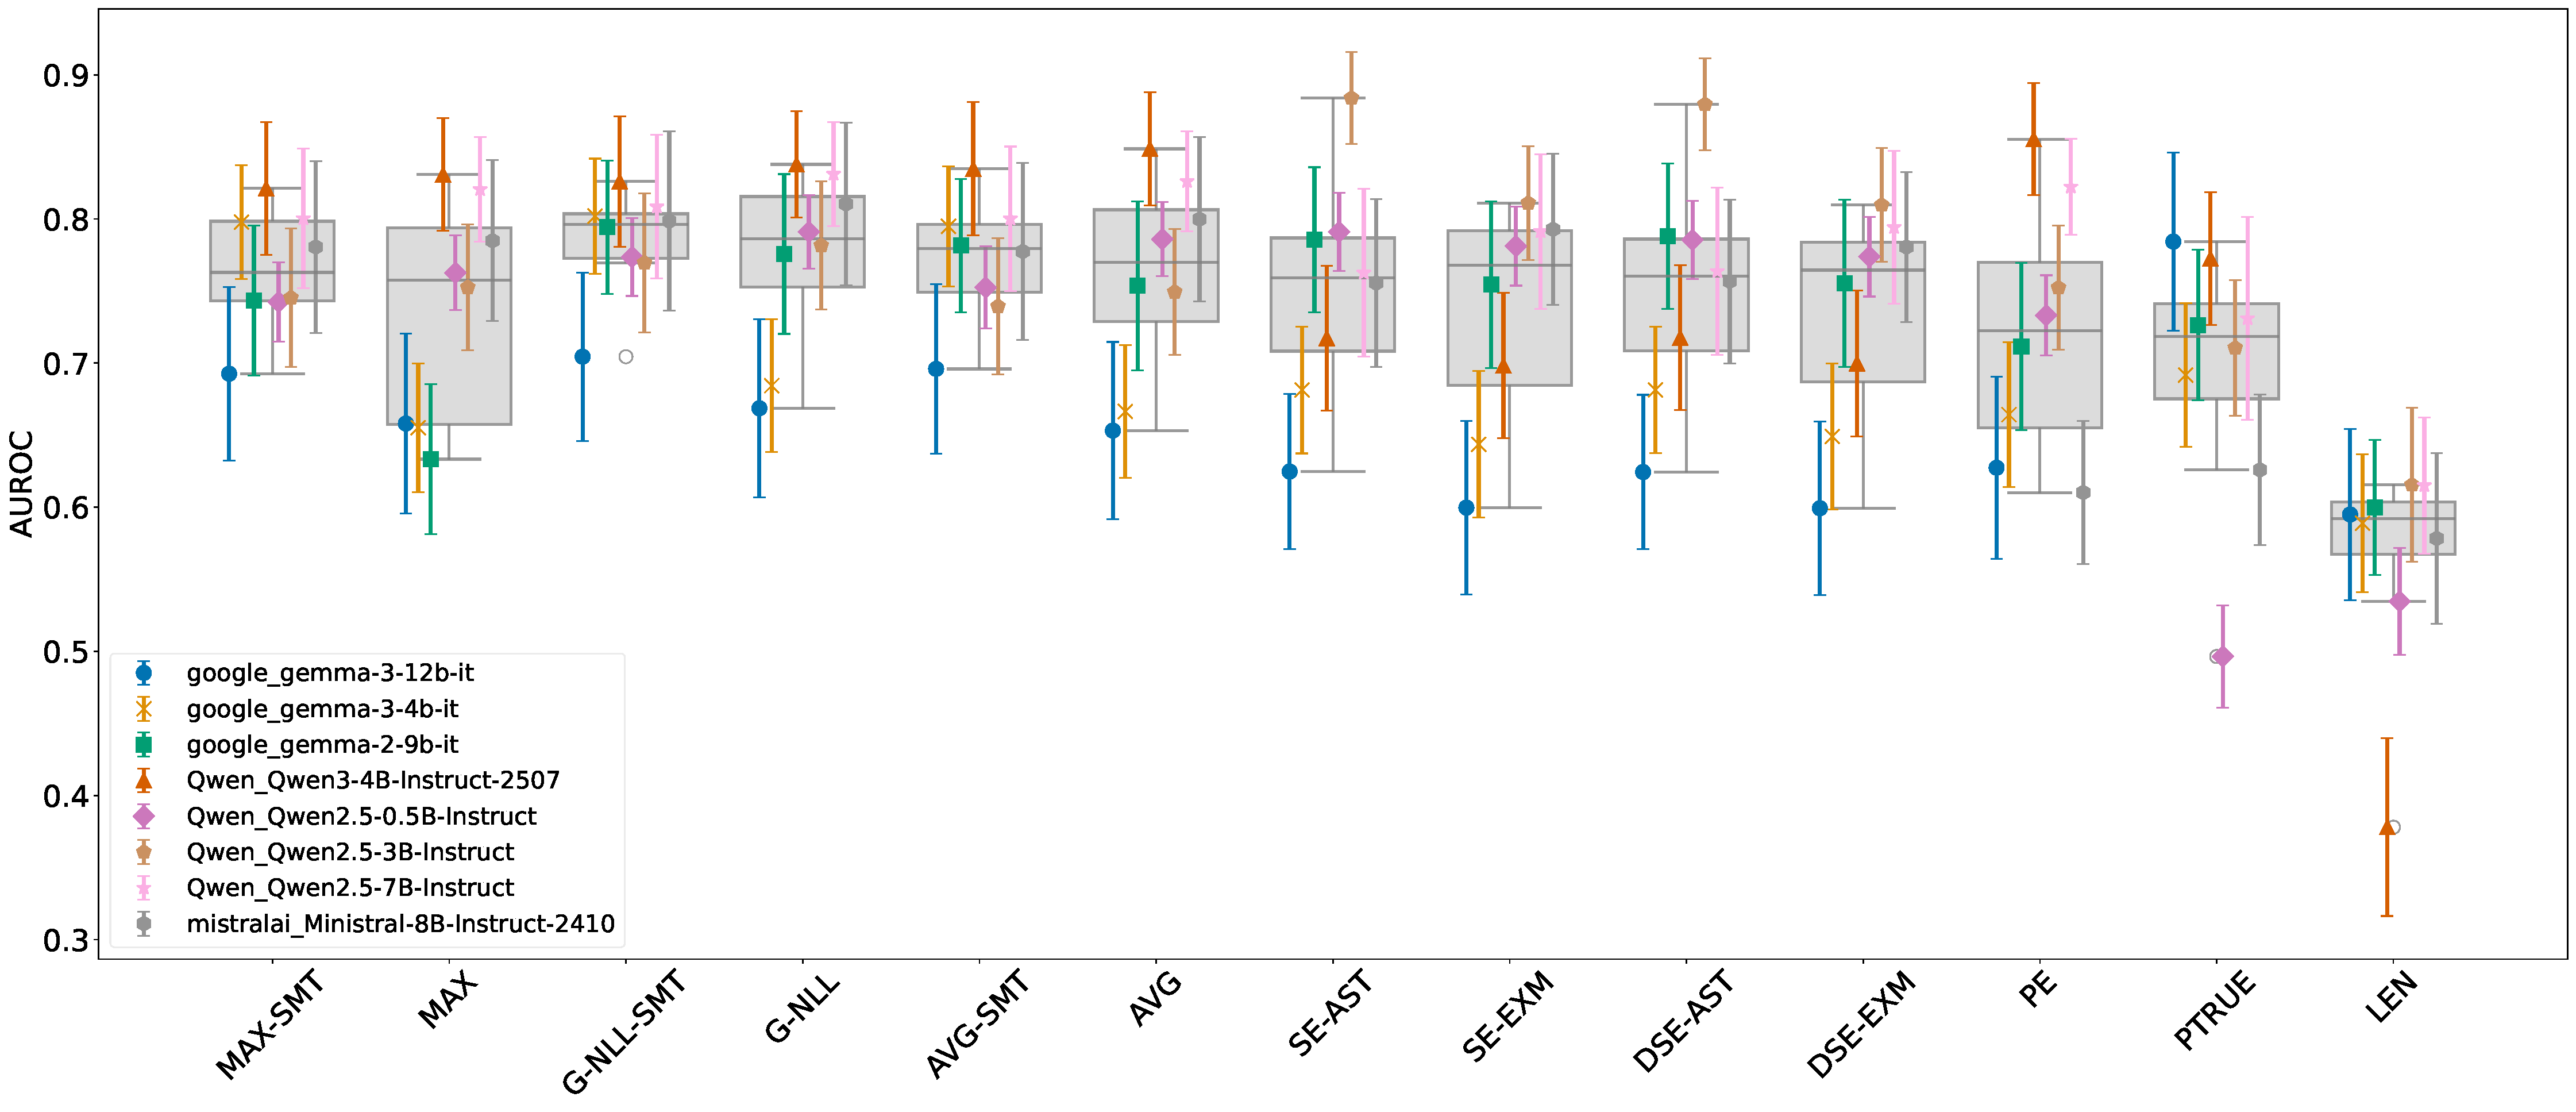
\includegraphics[width=\textwidth]{figures/boxplots/simple_boxplot.pdf}
        \caption{Simple}
        \label{fig:Simple}
    \end{subfigure}
    \hfill
    \begin{subfigure}[c]{0.48\textwidth}
        \centering
        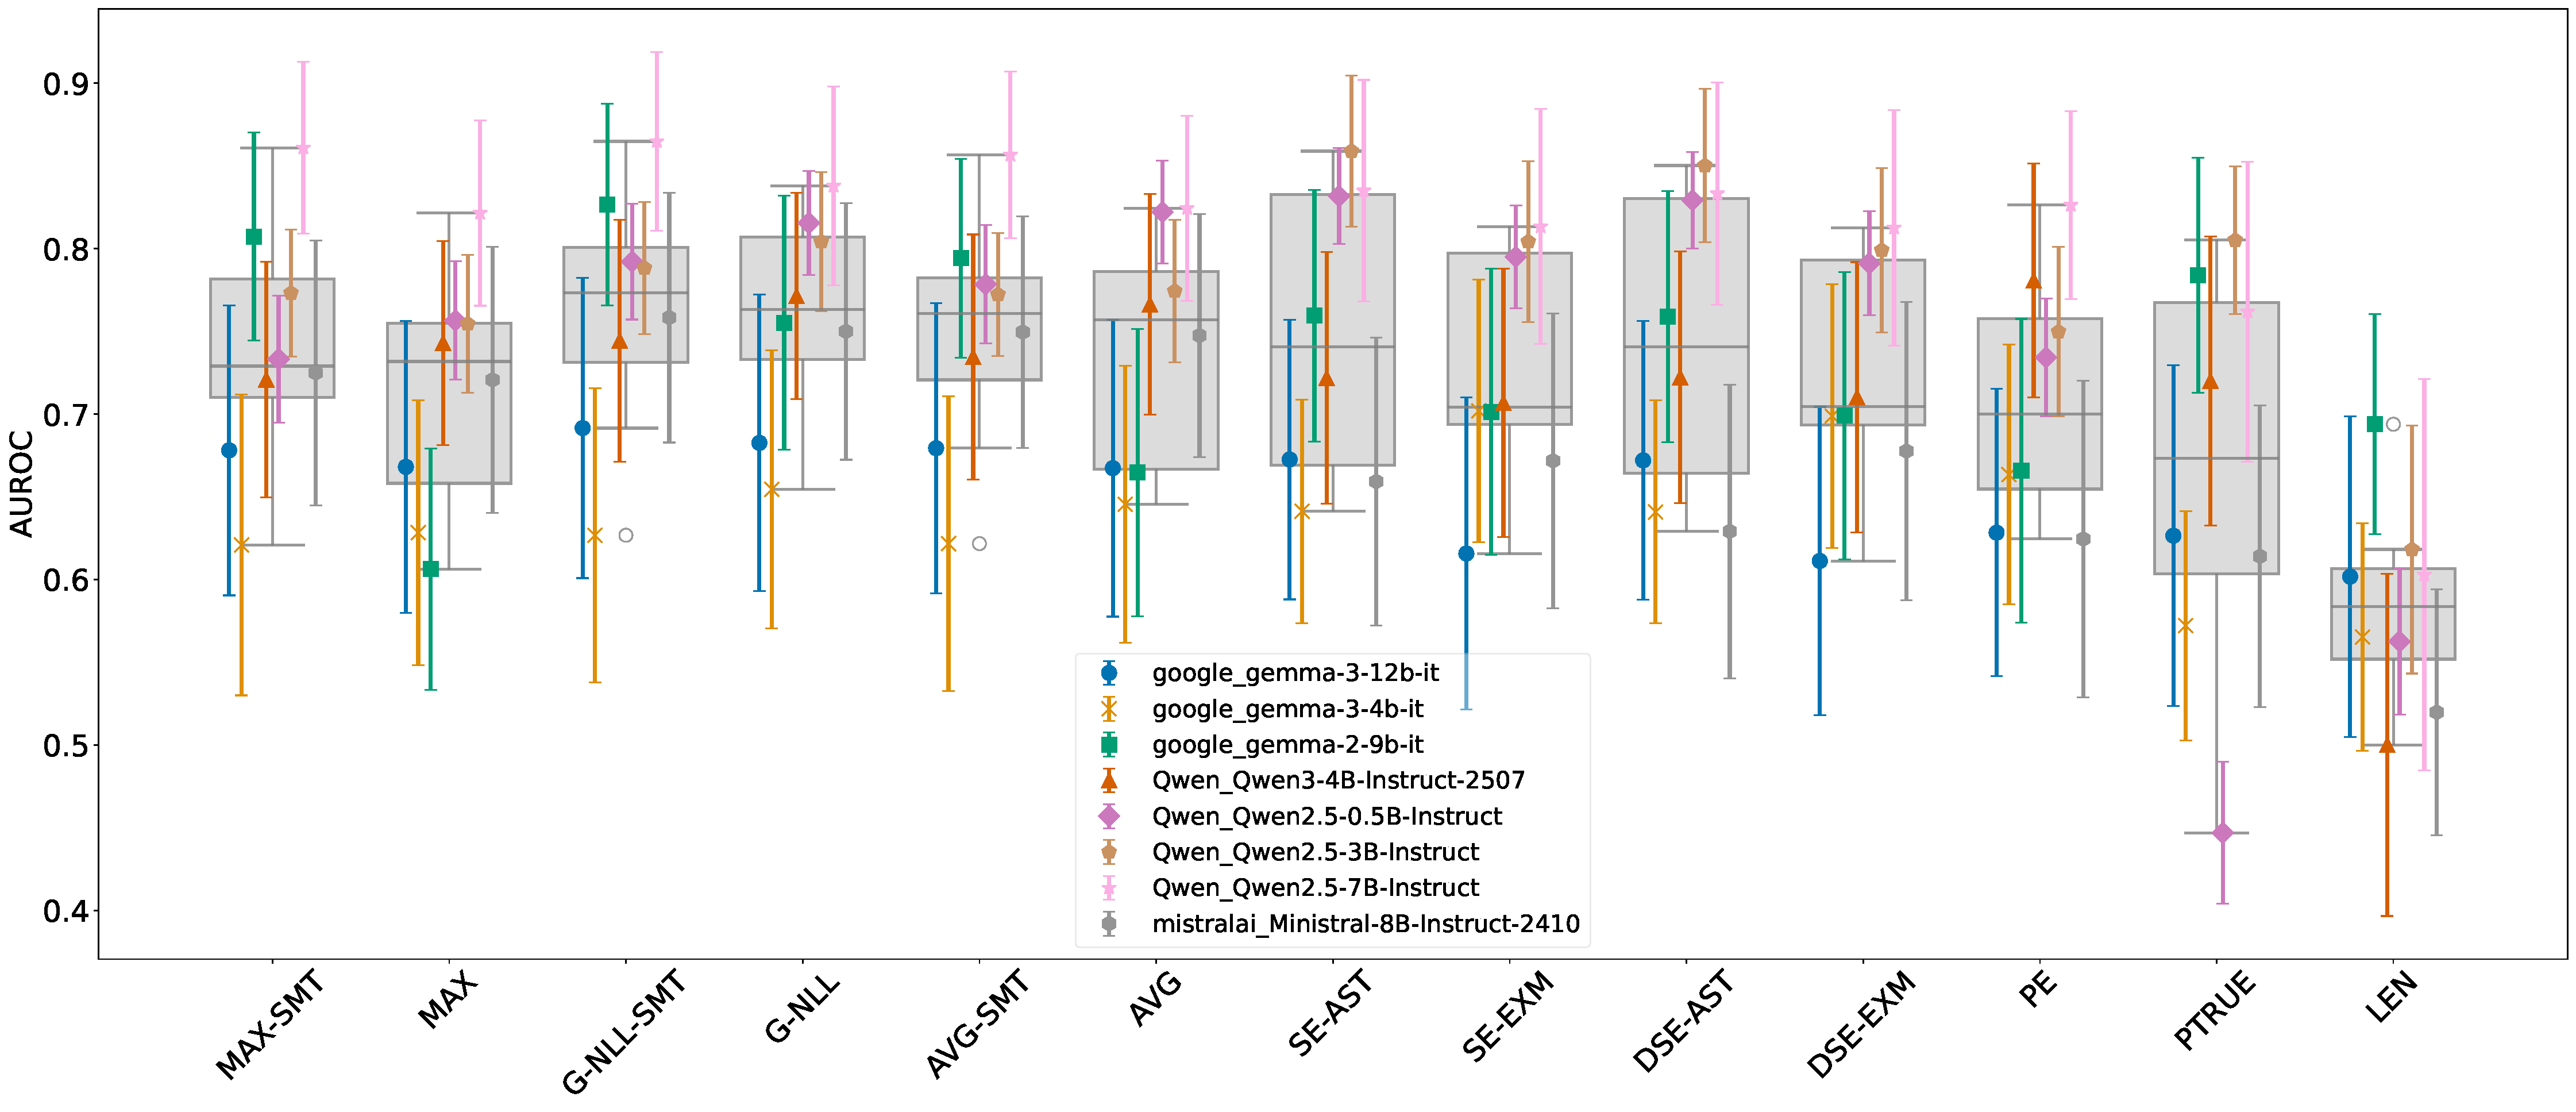
\includegraphics[width=\textwidth]{figures/boxplots/multiple_boxplot.pdf}
        \caption{Multiple}
        \label{fig:Multiple}
    \end{subfigure}

    \vskip\baselineskip

    \begin{subfigure}[c]{0.48\textwidth}
        \centering
        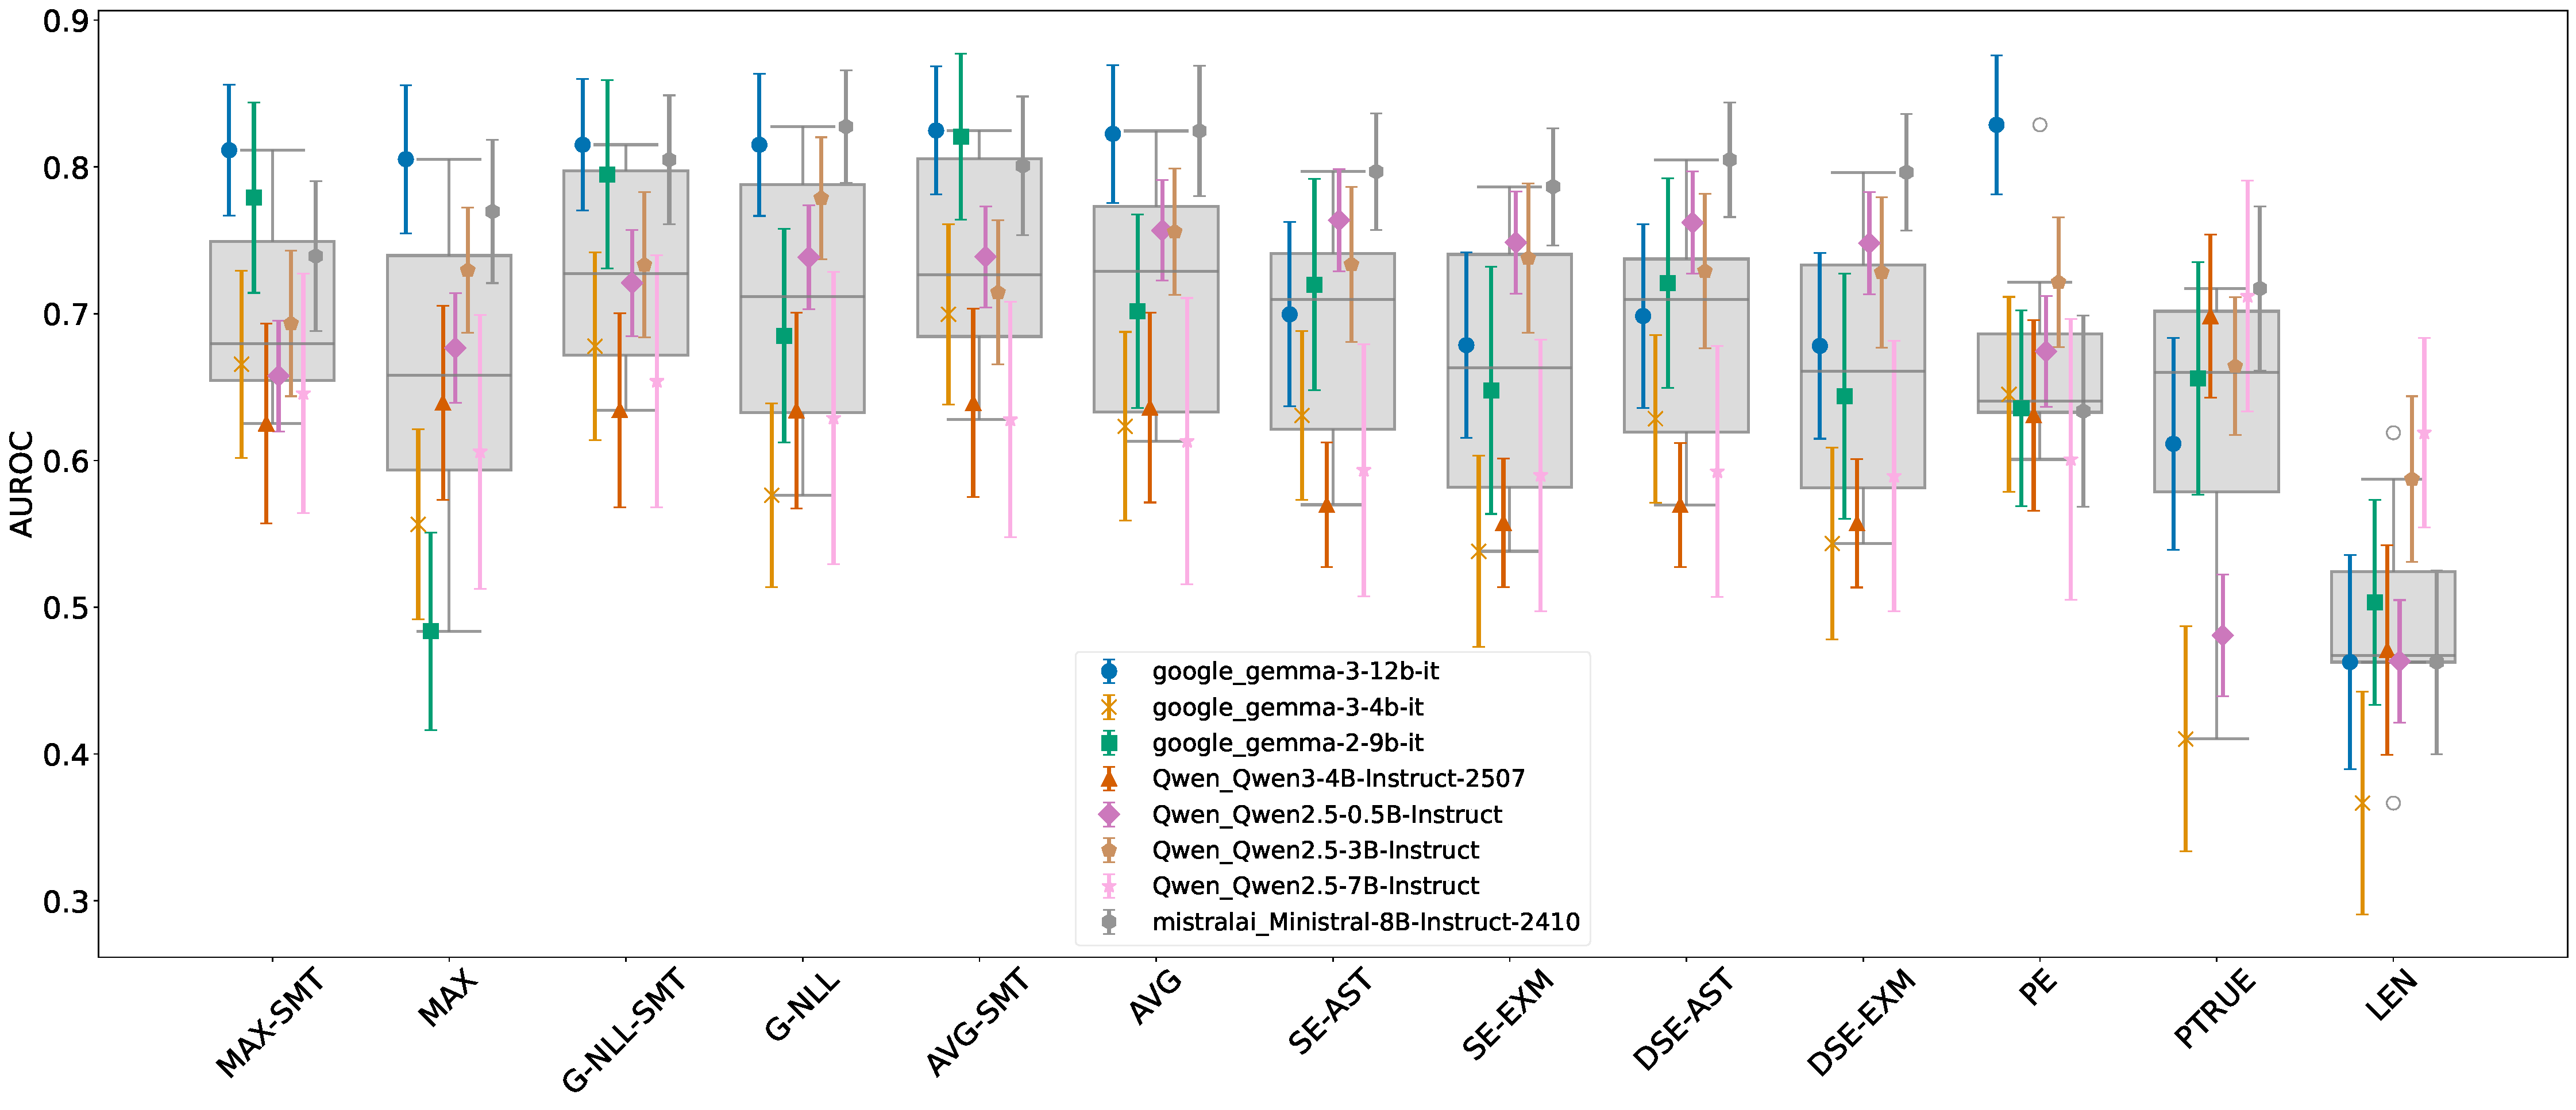
\includegraphics[width=\textwidth]{figures/boxplots/parallel_boxplot.pdf}
        \caption{Parallel}
        \label{fig:Parallel}
    \end{subfigure}
    \hfill
    \begin{subfigure}[c]{0.48\textwidth}
        \centering
        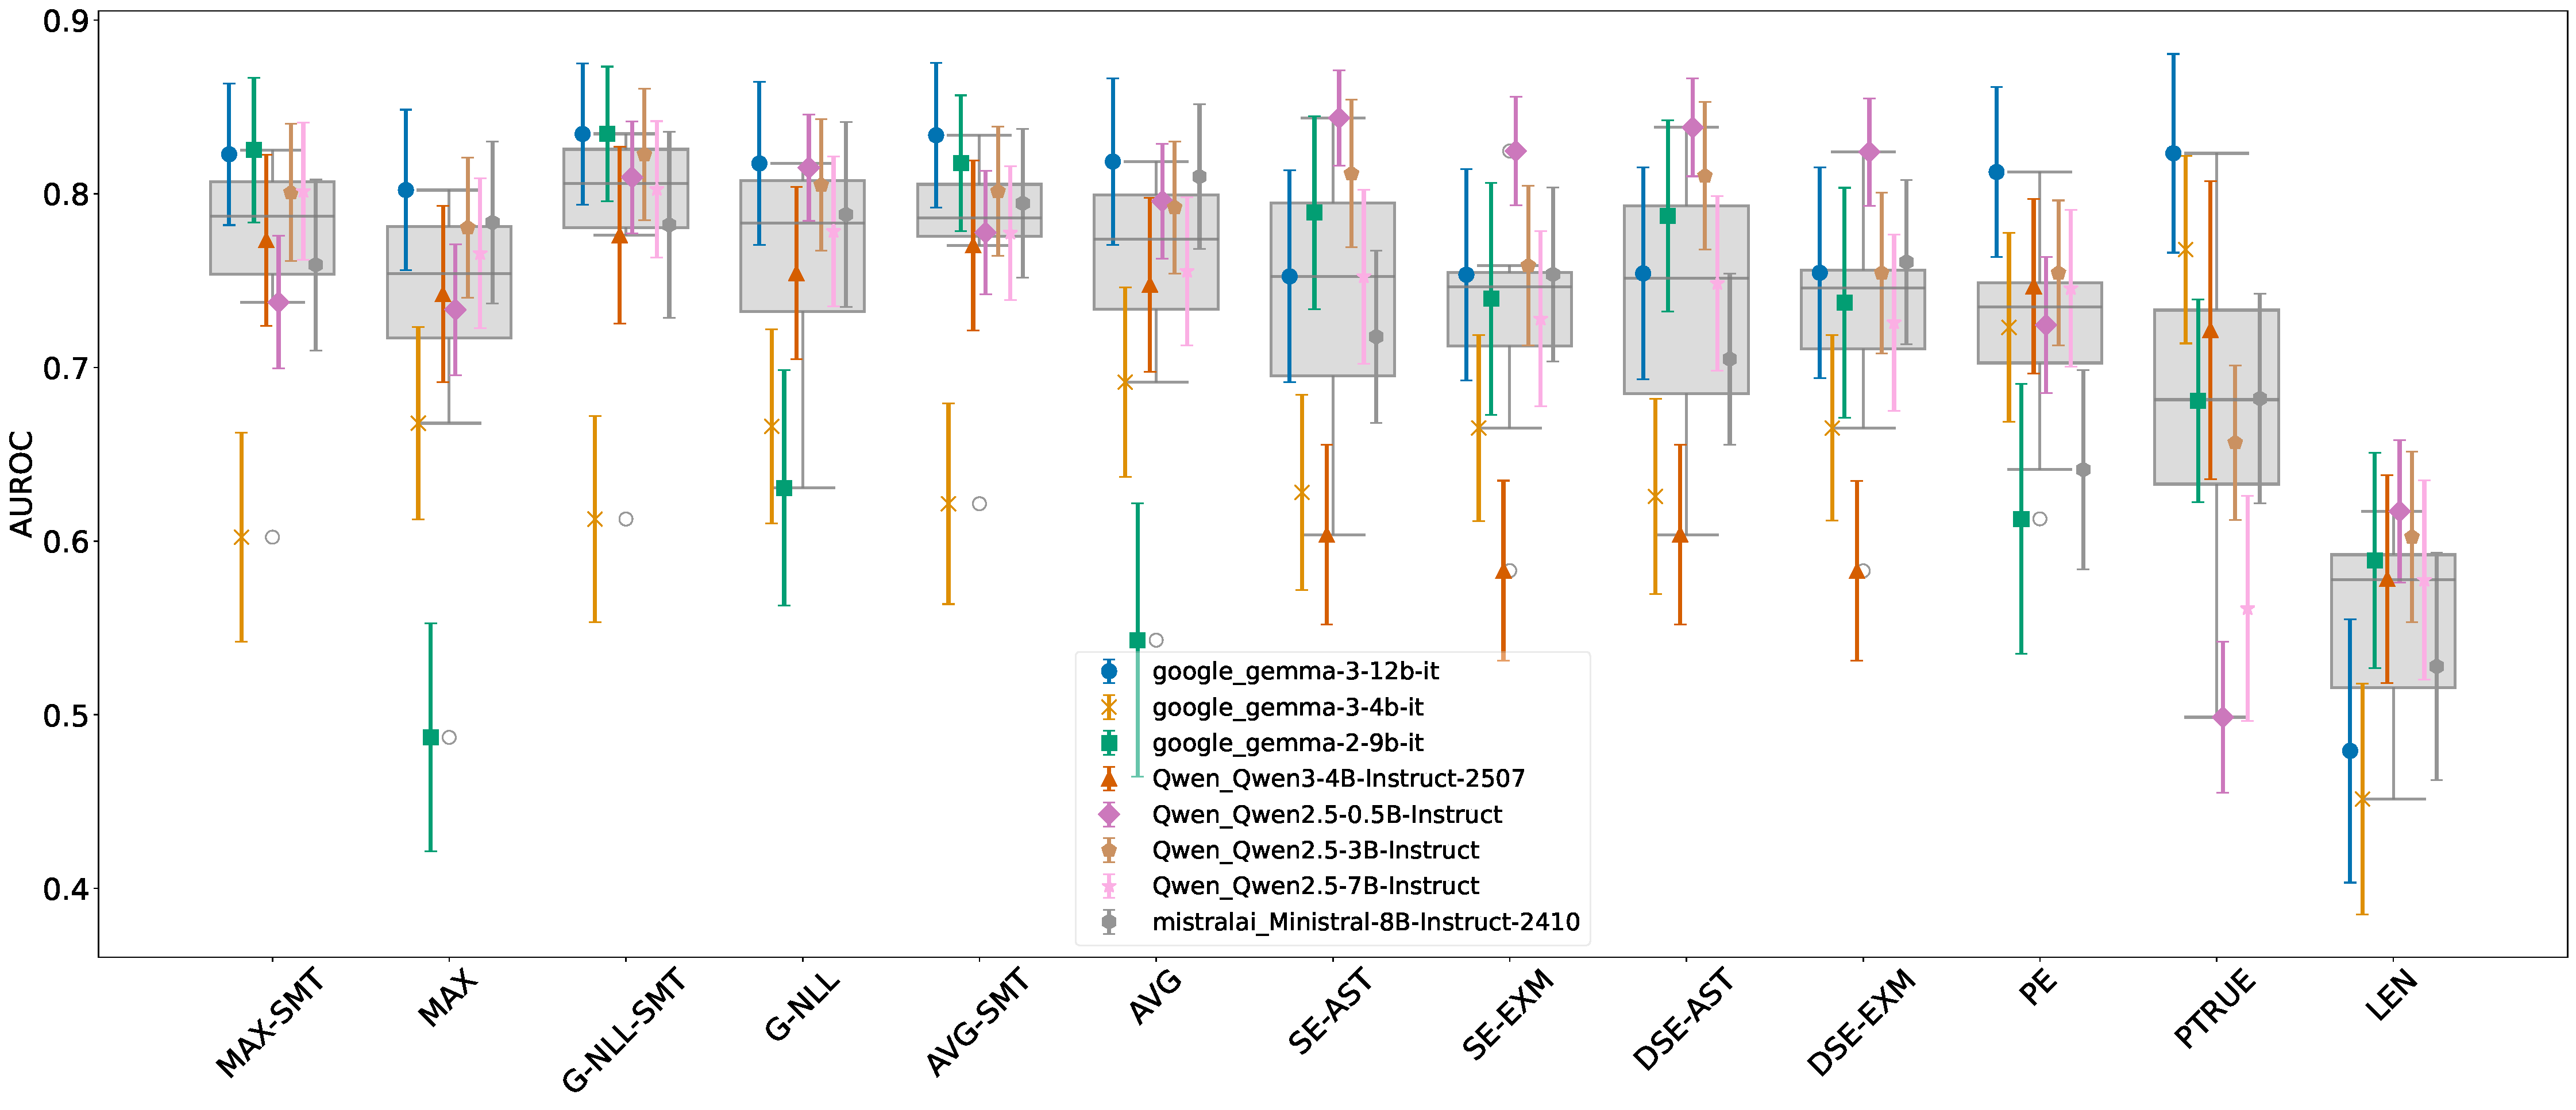
\includegraphics[width=\textwidth]{figures/boxplots/parallel_multiple_boxplot.pdf}
        \caption{Parallel-Multiple}
        \label{fig:Parallel-Multiple}
    \end{subfigure}

    \caption{
        Individual tasks:
        AUROC $\pm$ standard error (bootstrap estimate with $n=1000$) for the individual tasks described in \Cref{sec:individual_tasks}. Boxplots summarize the variation across LLMs.
    }
    \label{fig:individual_tasks}
\end{figure*}


\begin{figure*}[h!]
    \centering
    \begin{subfigure}[c]{0.48\textwidth}
        \centering
        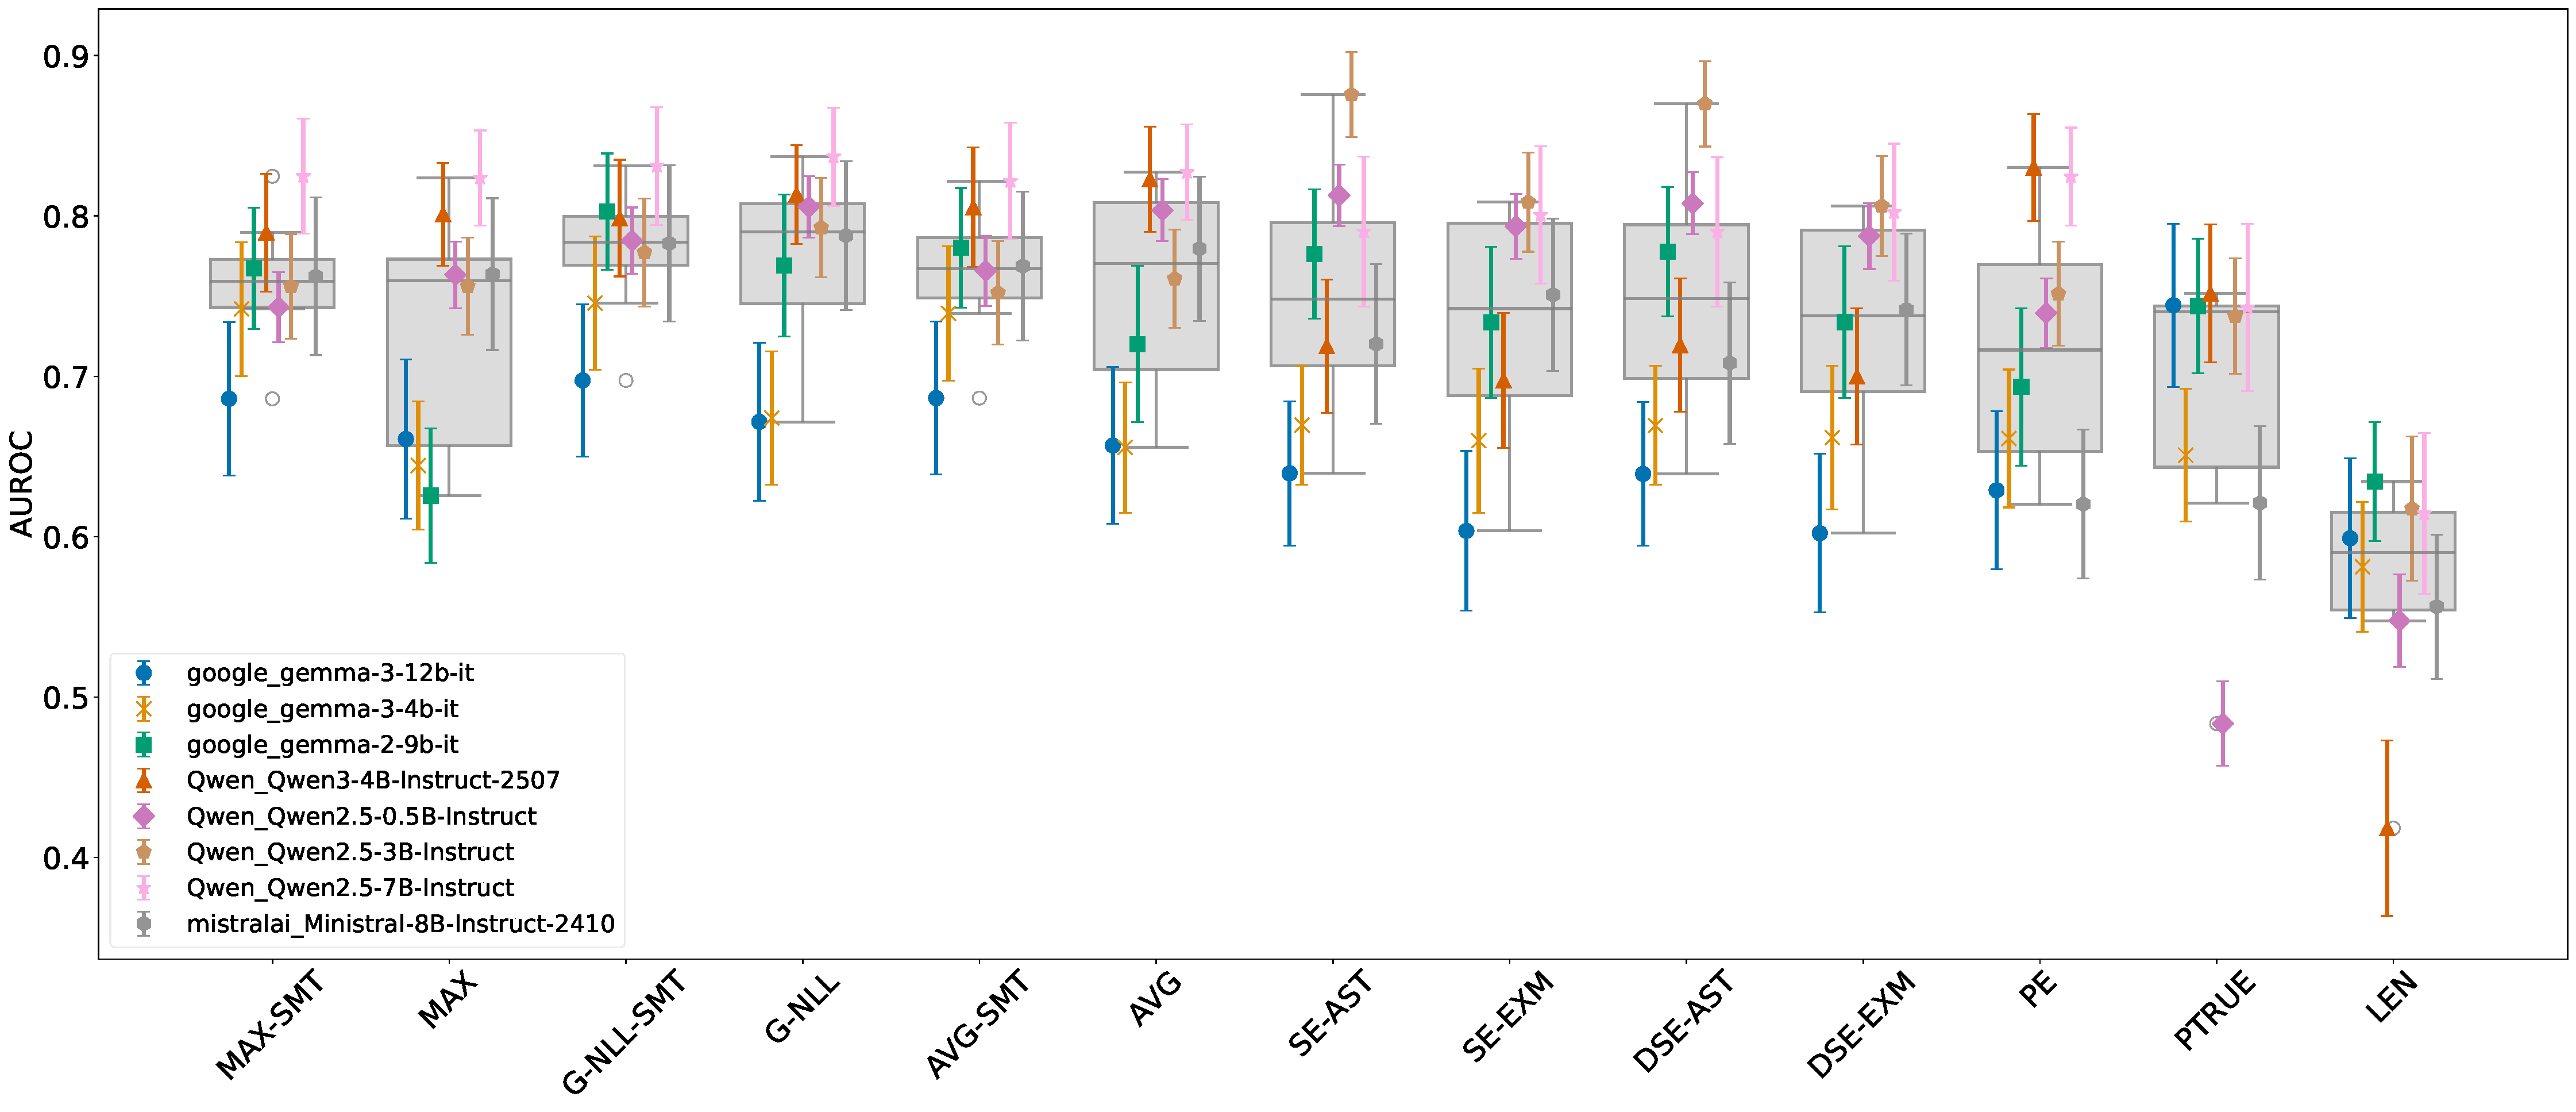
\includegraphics[width=\textwidth]{figures/boxplots/simple-multiple_boxplot.pdf}
        \caption{Simple + Multiple}
        \label{fig:Simple+Multiple}
    \end{subfigure}
    \hfill
    \begin{subfigure}[c]{0.48\textwidth}
        \centering
        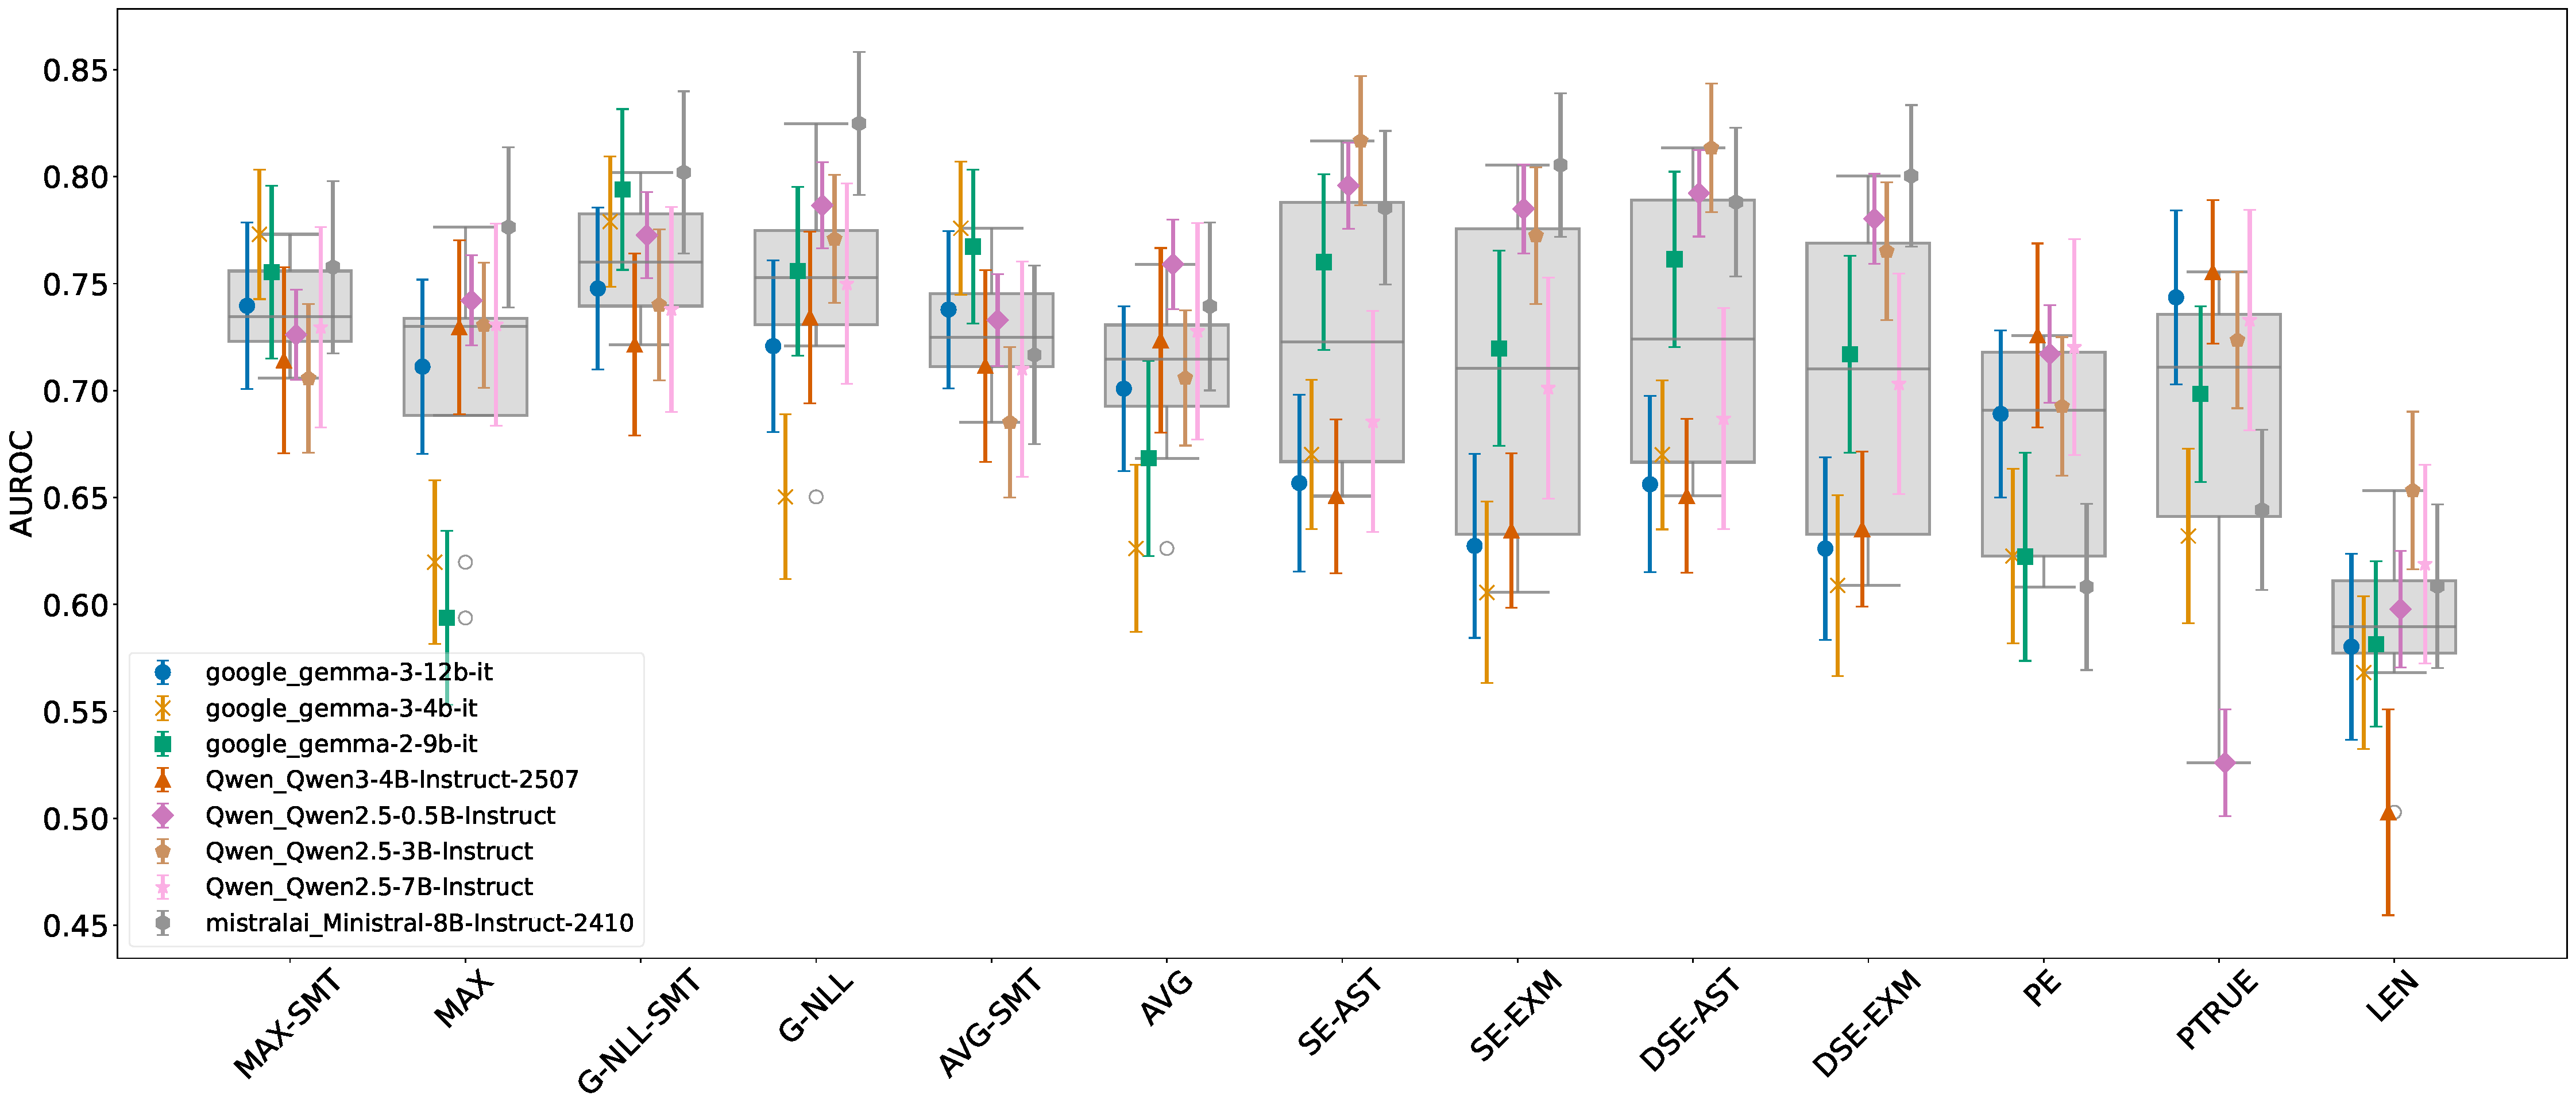
\includegraphics[width=\textwidth]{figures/boxplots/simple-parallel_boxplot.pdf}
        \caption{Simple + Parallel}
        \label{fig:Simple+Parallel}
    \end{subfigure}

    \vspace{0.5em}

    \begin{subfigure}[c]{0.48\textwidth}
        \centering
        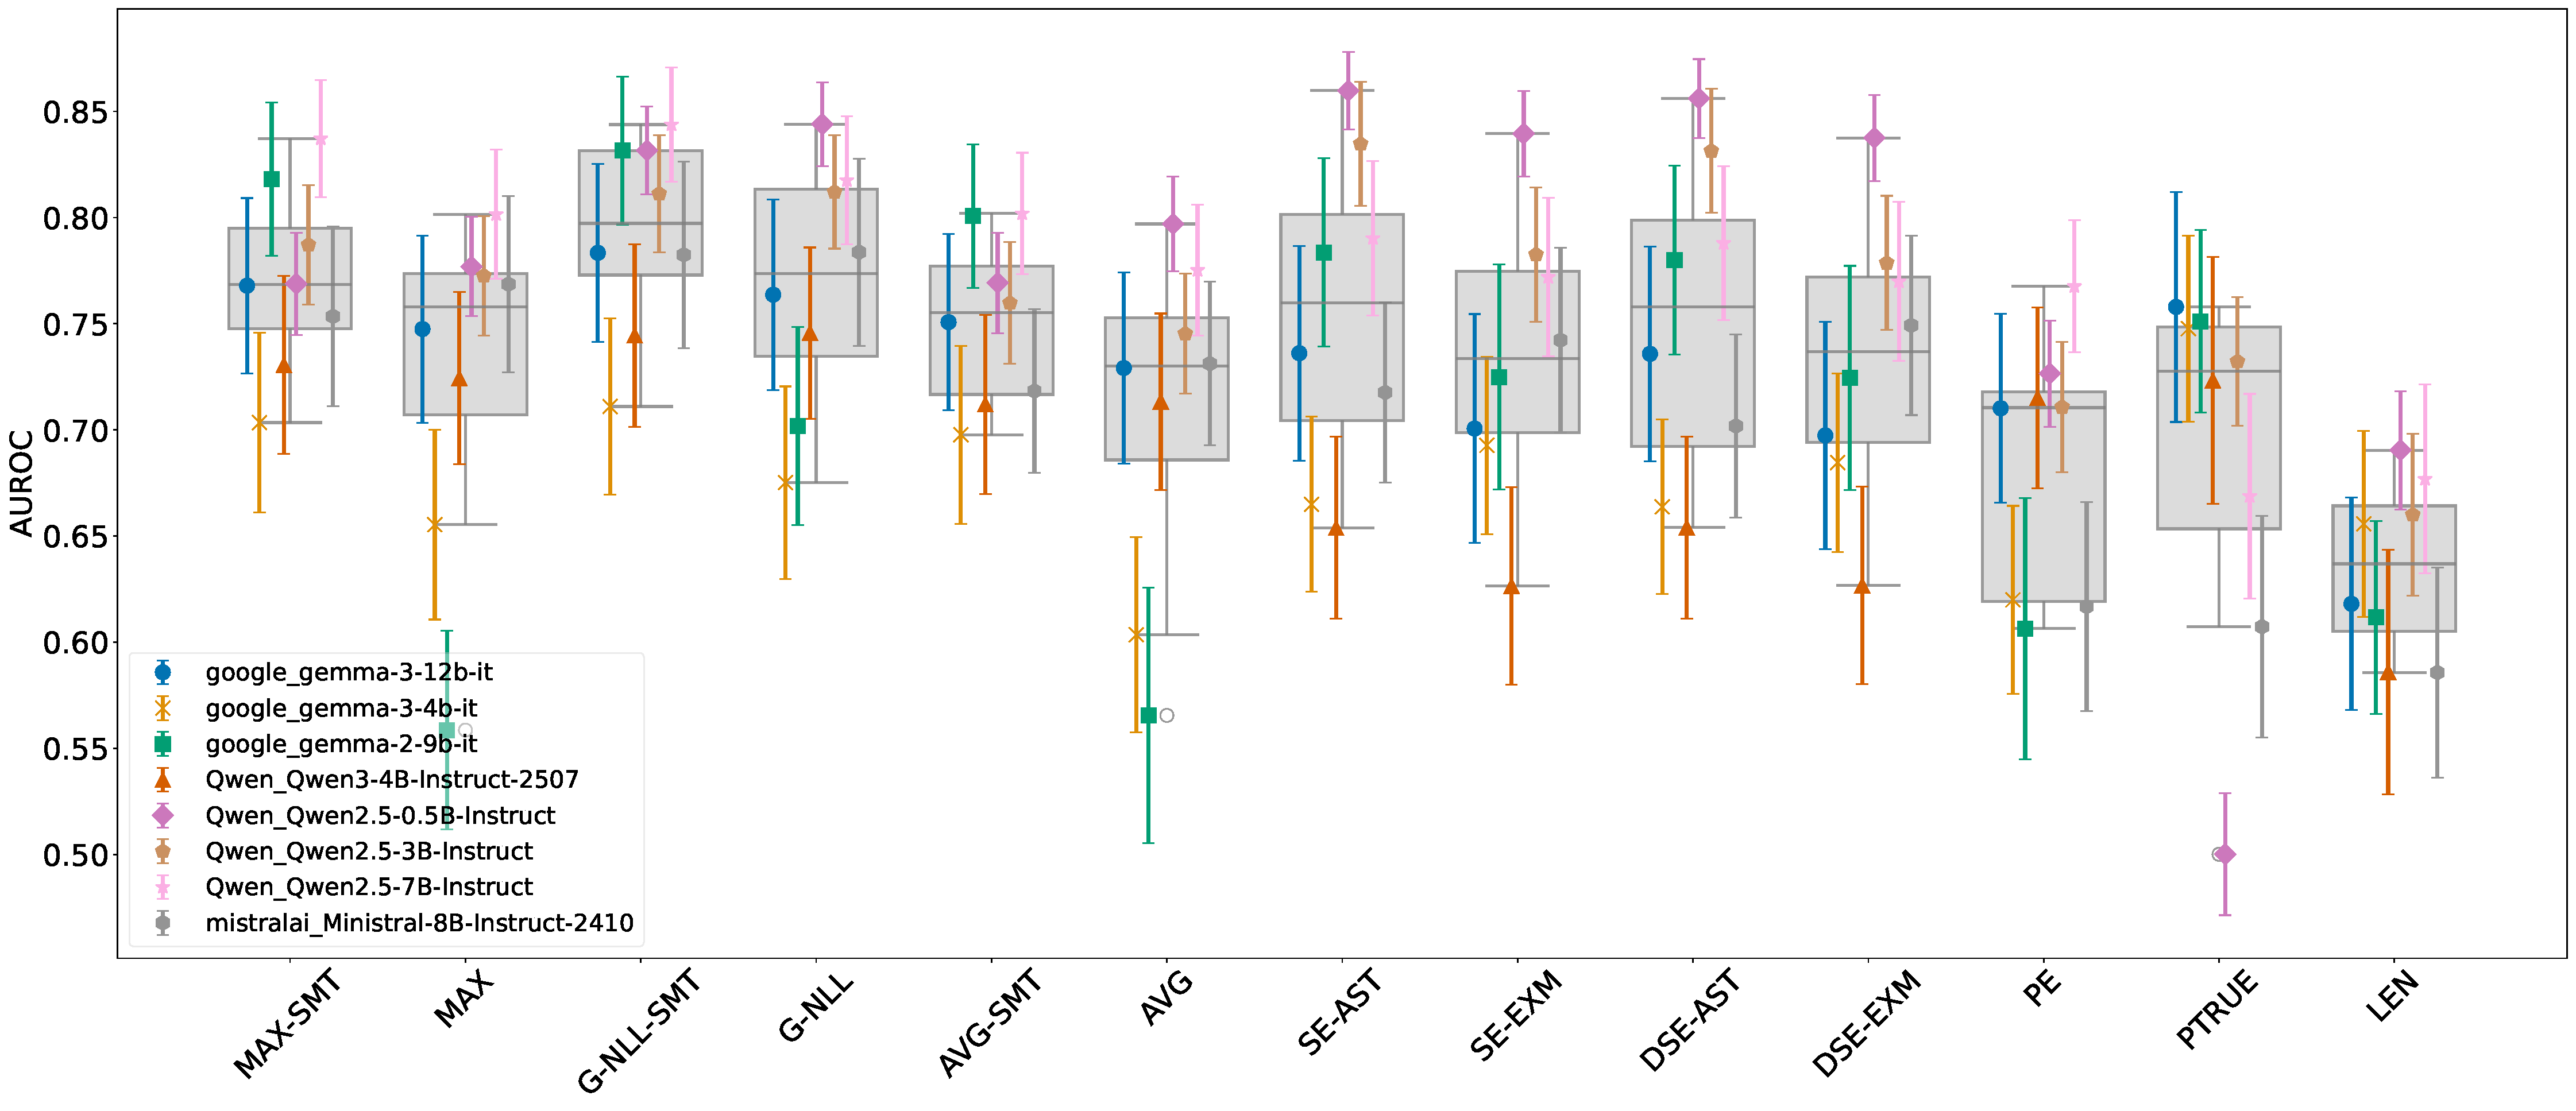
\includegraphics[width=\textwidth]{figures/boxplots/multiple-parallel_multiple_boxplot.pdf}
        \caption{Multiple + \mbox{Parallel-Multiple}}
        \label{fig:Multiple+Parallel-Multiple}
    \end{subfigure}
    \hfill
    \begin{subfigure}[c]{0.48\textwidth}
        \centering
        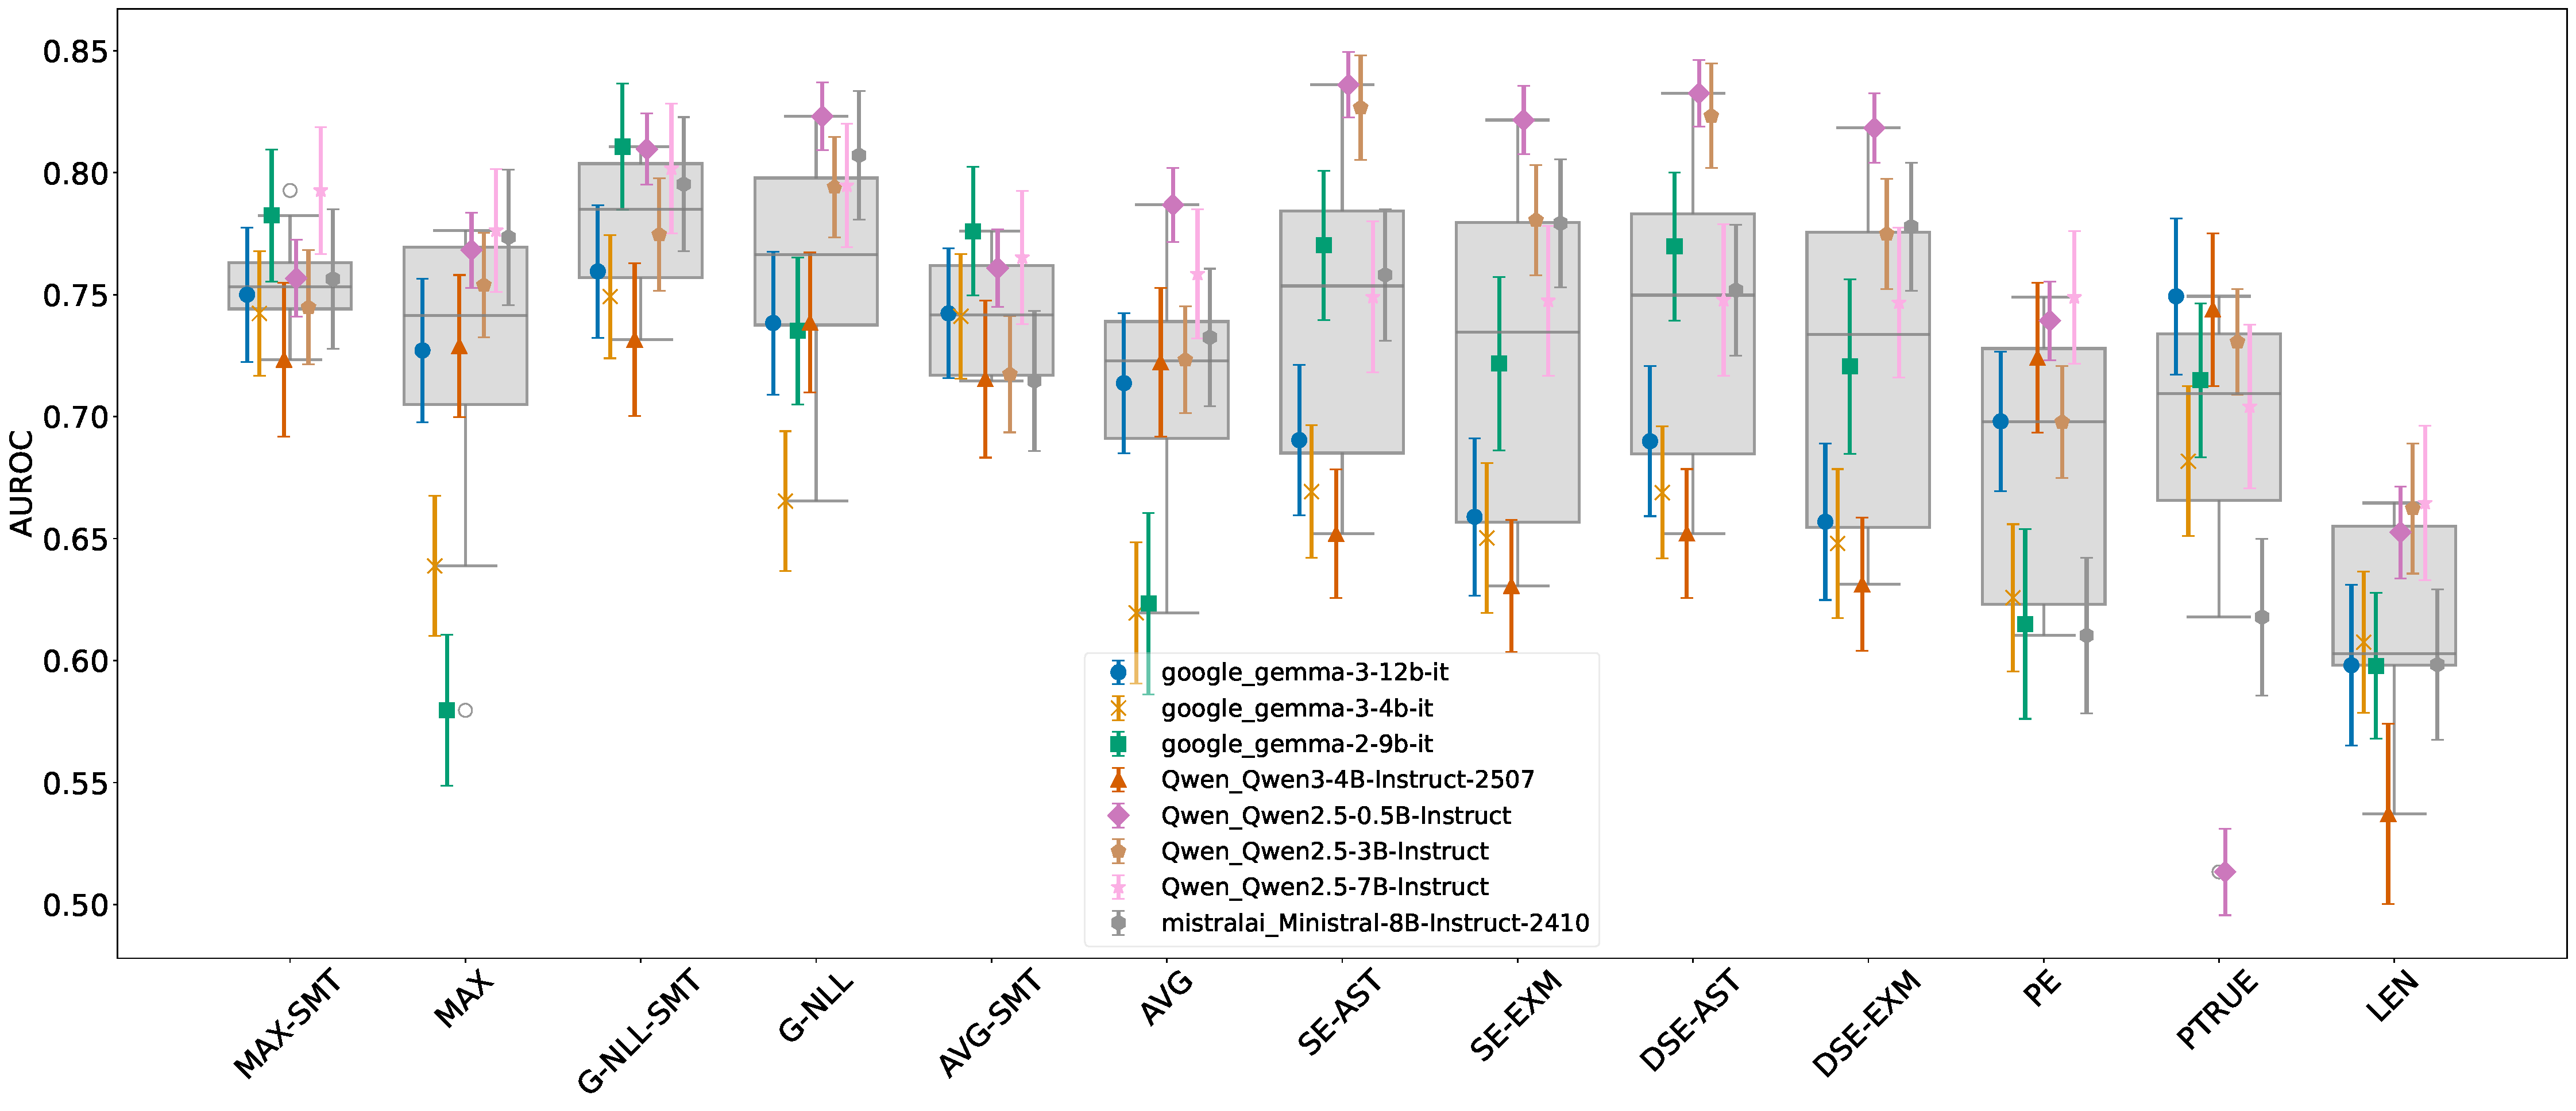
\includegraphics[width=\textwidth]{figures/boxplots/simple-multiple-parallel-parallel_multiple_boxplot.pdf}
        \caption{All Combined}
        \label{fig:All}
    \end{subfigure}

    \caption{
        Combinations of tasks: 
        AUROC $\pm$ std.\ error for the combinations of tasks described in \Cref{sec:combinations}. Boxplots summarize the variation across LLMs for a given UQ method.
    }
    \label{fig:combinations}
\end{figure*}







\begin{figure*}[h!]
\centering
    \begin{subfigure}[c]{0.48\textwidth}
        \centering
        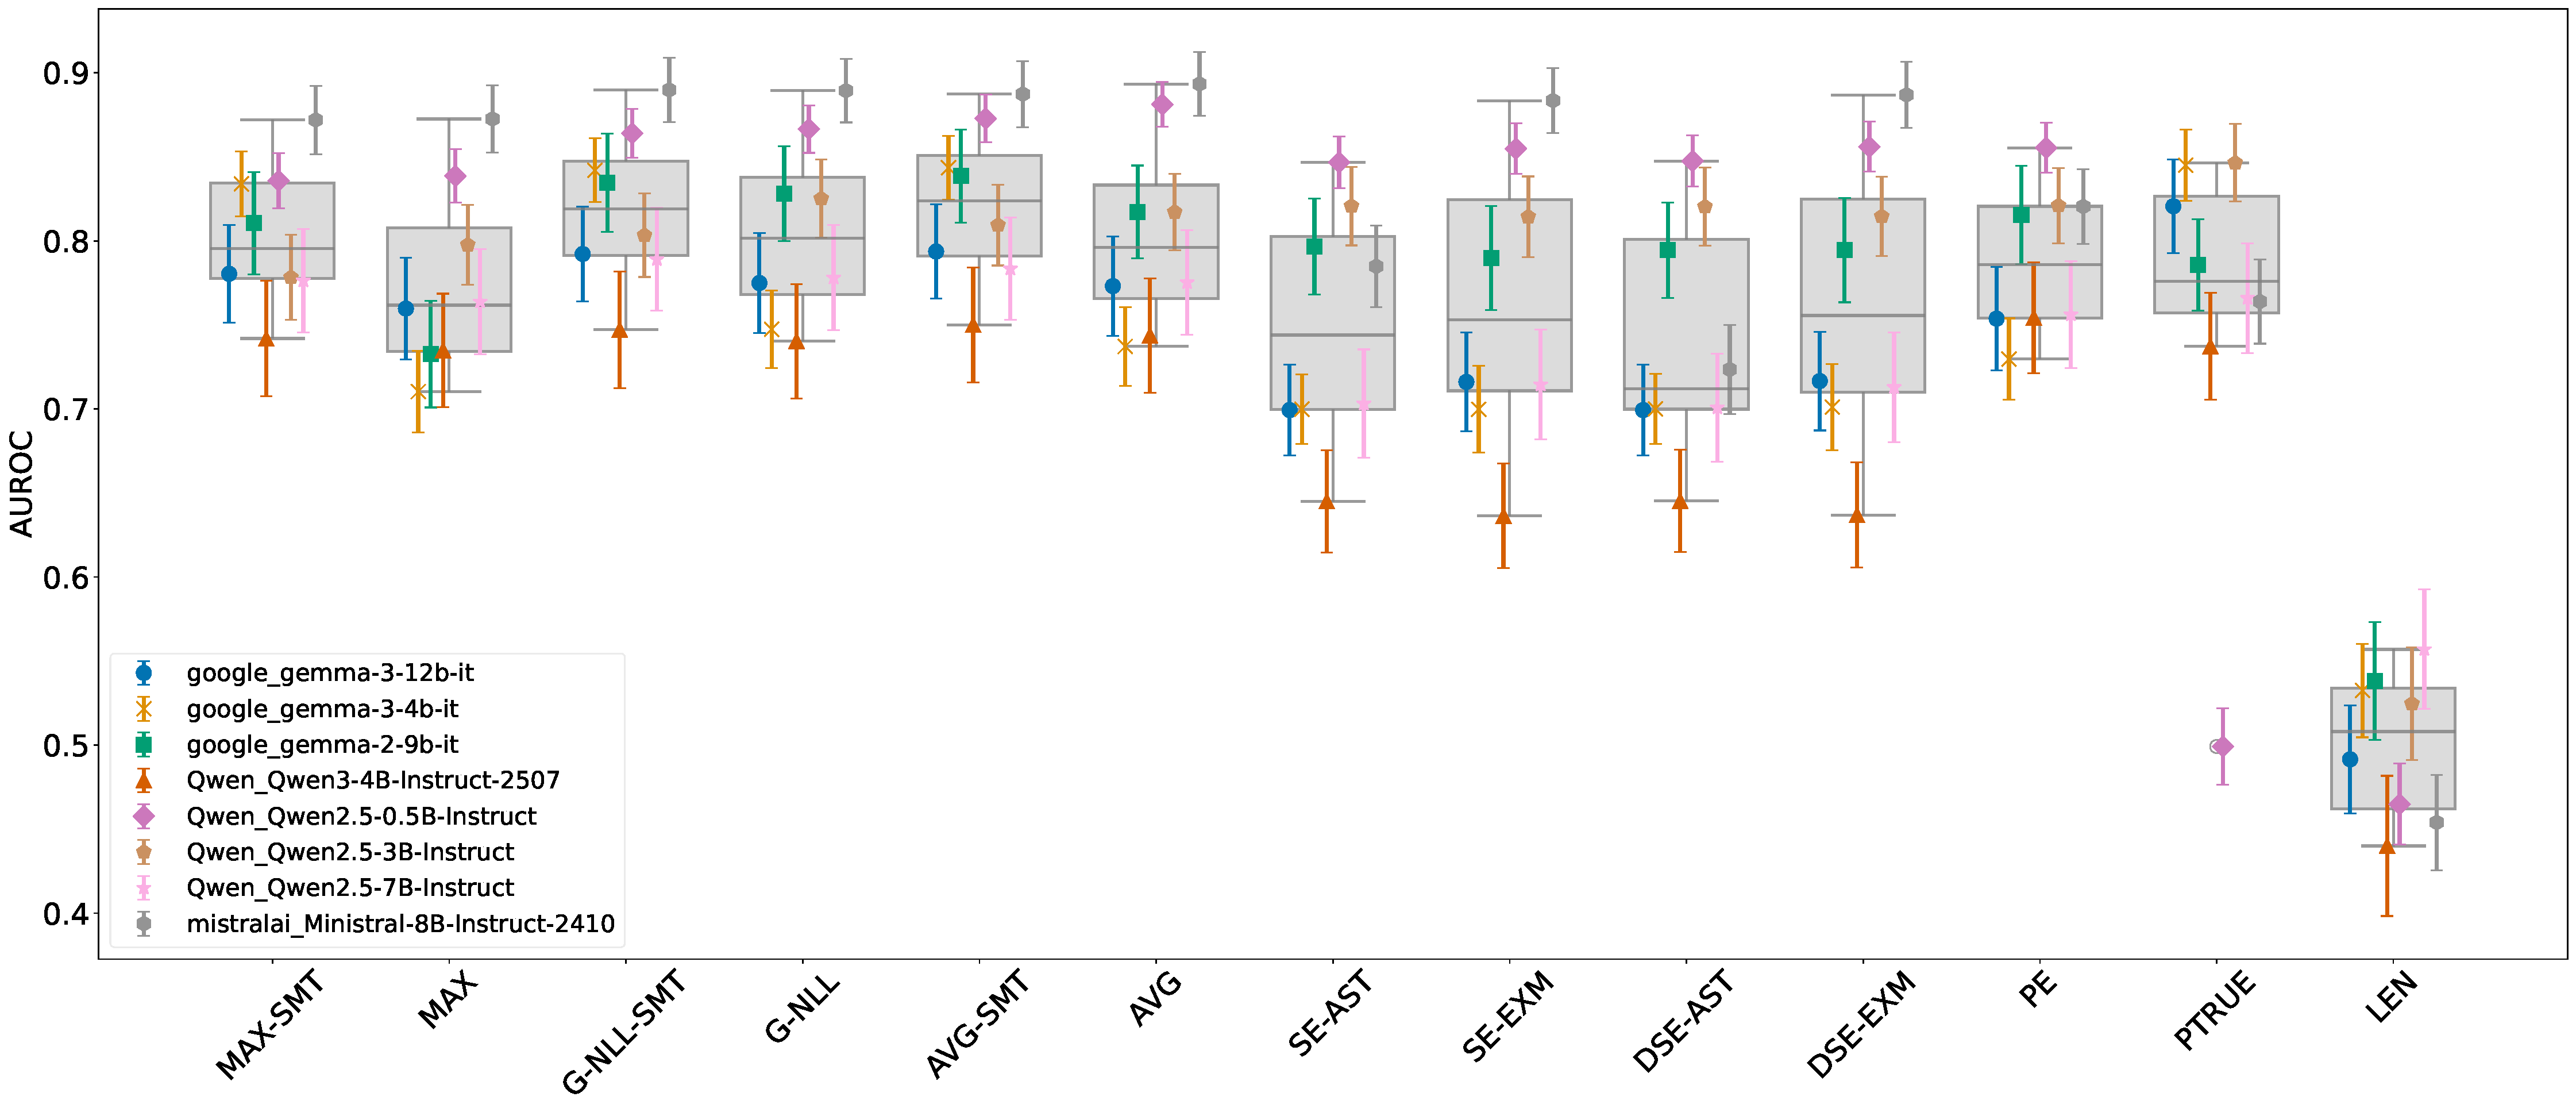
\includegraphics[width=\textwidth]{figures/boxplots/simple-irrelevance_boxplot.pdf}
        \caption{Simple + Irrelevance}
        \label{fig:Simple+Irrelevance}
    \end{subfigure}
    \hfill
    \begin{subfigure}[c]{0.48\textwidth}
        \centering
        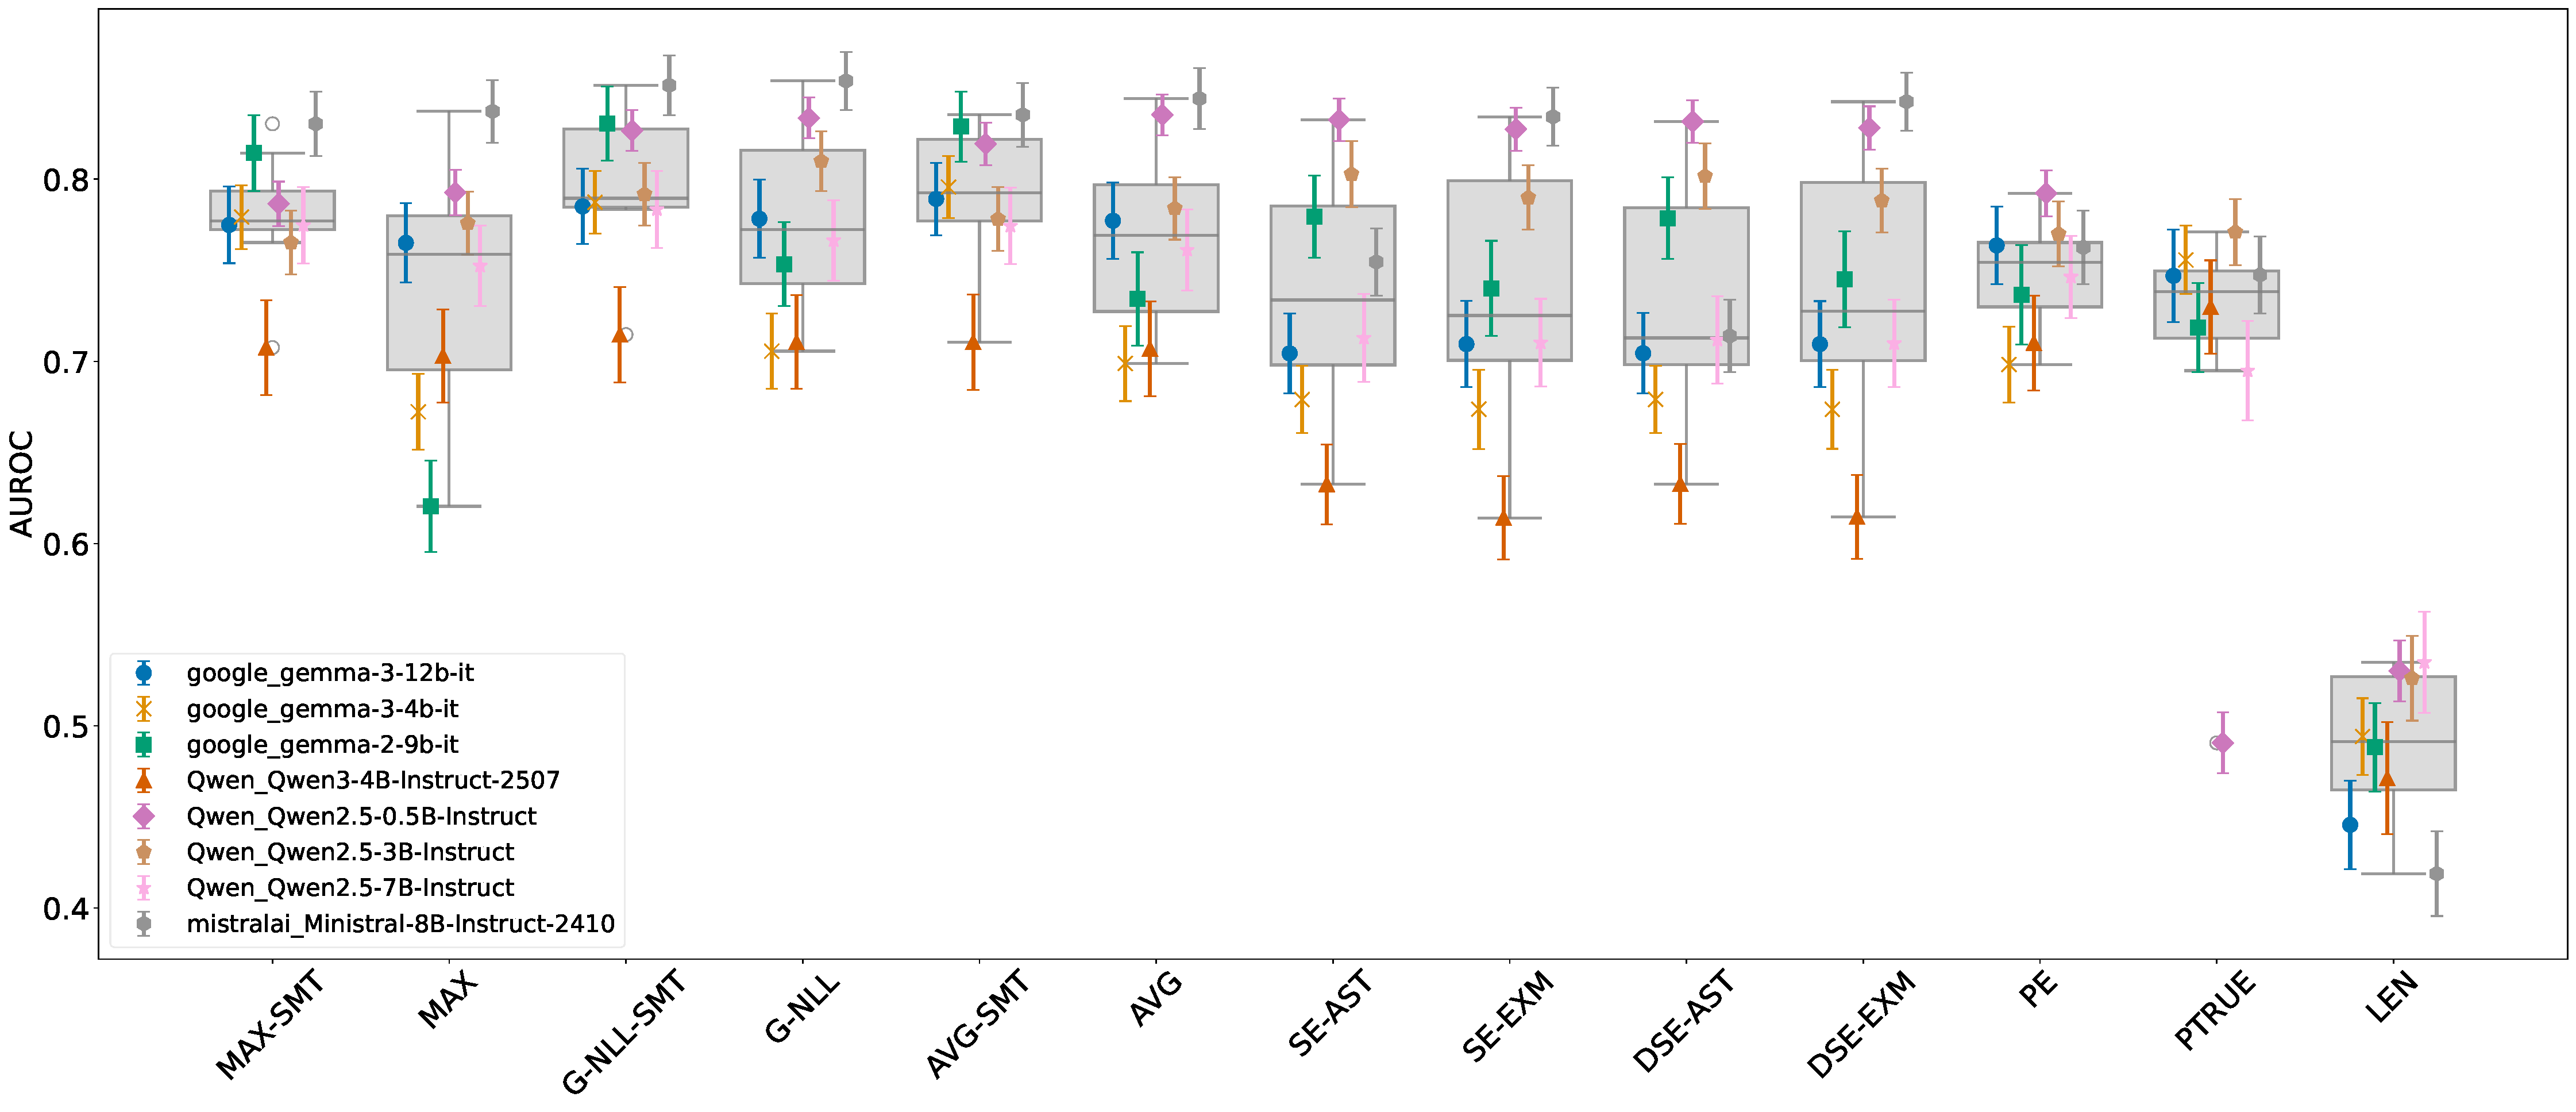
\includegraphics[width=\textwidth]{figures/boxplots/simple-multiple-parallel-parallel_multiple-irrelevance_boxplot.pdf}
        \caption{All Combined + Irrelevance}
        \label{fig:All+Irrelevance}
    \end{subfigure}

    \caption{
        Unanswerable requests: 
        AUROC $\pm$ standard error for the combinations of answerable and unanswerable tasks described in \Cref{sec:irrelevance_combinations}. Boxplots summarize the variation across LLMs for a given UQ method.
    }
    \label{fig:irrelevance_combinations}
\end{figure*}


\subsection{Risk-Coverage Curves}
\label{sec:risk_coverage}


As an additional analysis, we include the risk-coverage curves (averaged across models) for the individual tasks in \Cref{fig:individual_tasks_riskcoverage}, for the combined tasks in \Cref{fig:combined_tasks_riskcoverage}, and for the combinations that also include the irrelevance split in \Cref{fig:irrelevance_combinations_riskcoverage}.

We see that indeed, UQ methods can be used to achieve higher accuracy through abstention. For example, not executing a function call for the 30\% of requests with highest G-NLL$_{SMT}$ UQ scores in their output, the accuracies increase from $<92 \%$ to $96 \%$  for \emph{Simple}, from $90 \%$ to $95 \%$ for \emph{Multiple}, from $84 \%$ to $90 \%$ for \emph{Parallel}, and from $79 \%$ to $86 \%$ for \emph{Parallel-Multiple} (\Cref{fig:individual_tasks_riskcoverage}). The gains are similar for the combinations of tasks, and even reach $\approx +10 \%$ once the irrelevance task is added (from $75 \%$ to $85 \%$ and $80\%$ to $90 \%$ in \Cref{fig:irrelevance_combinations_riskcoverage}). 
If one only executes the function calls with the lowest $10 \%$ of G-NLL$_{SMT}$ uncertainty scores, accuracies that can be reached are even higher: $ \approx 98 \%$ for  \emph{Simple} and \emph{Multiple}, $95 \%$ for \emph{Parallel}, and $93 \%$ for \emph{Parallel-Multiple} (\Cref{fig:individual_tasks_riskcoverage}), or $97 \%$ on \emph{All Combined} (\Cref{fig:All_rc}) and $\approx 95 \%$ on the combinations including the irrelevance task (\Cref{fig:irrelevance_combinations_riskcoverage}).

Also, we see some differences by method. P$_{true}$ and LEN clearly lag behind, corresponding to their markedly lower AUROCs in \Cref{sec:benchmark}. Between the remaining methods, the differences are more nuanced. However, for most tasks, the curves for the single-sample methods (G-NLL and G-NLL$_{SMT}$) are above those of the multi-sample methods (SE$_{EXM}$ and SE$_{AST}$), again corresponding to the AUROC results in \Cref{sec:benchmark}. Also, especially for the first half of coverage (until $0.5$), the methods adjusted to the FC setting (G-NLL$_{SMT}$ and SE$_{AST}$) have higher curves than those of their generic counterparts. However, this difference typically disappears in the second half of coverage (from $0.5$ to $0.1$).



\begin{figure*}[h!]
    \centering
    \begin{subfigure}[c]{0.48\textwidth}
        \centering
        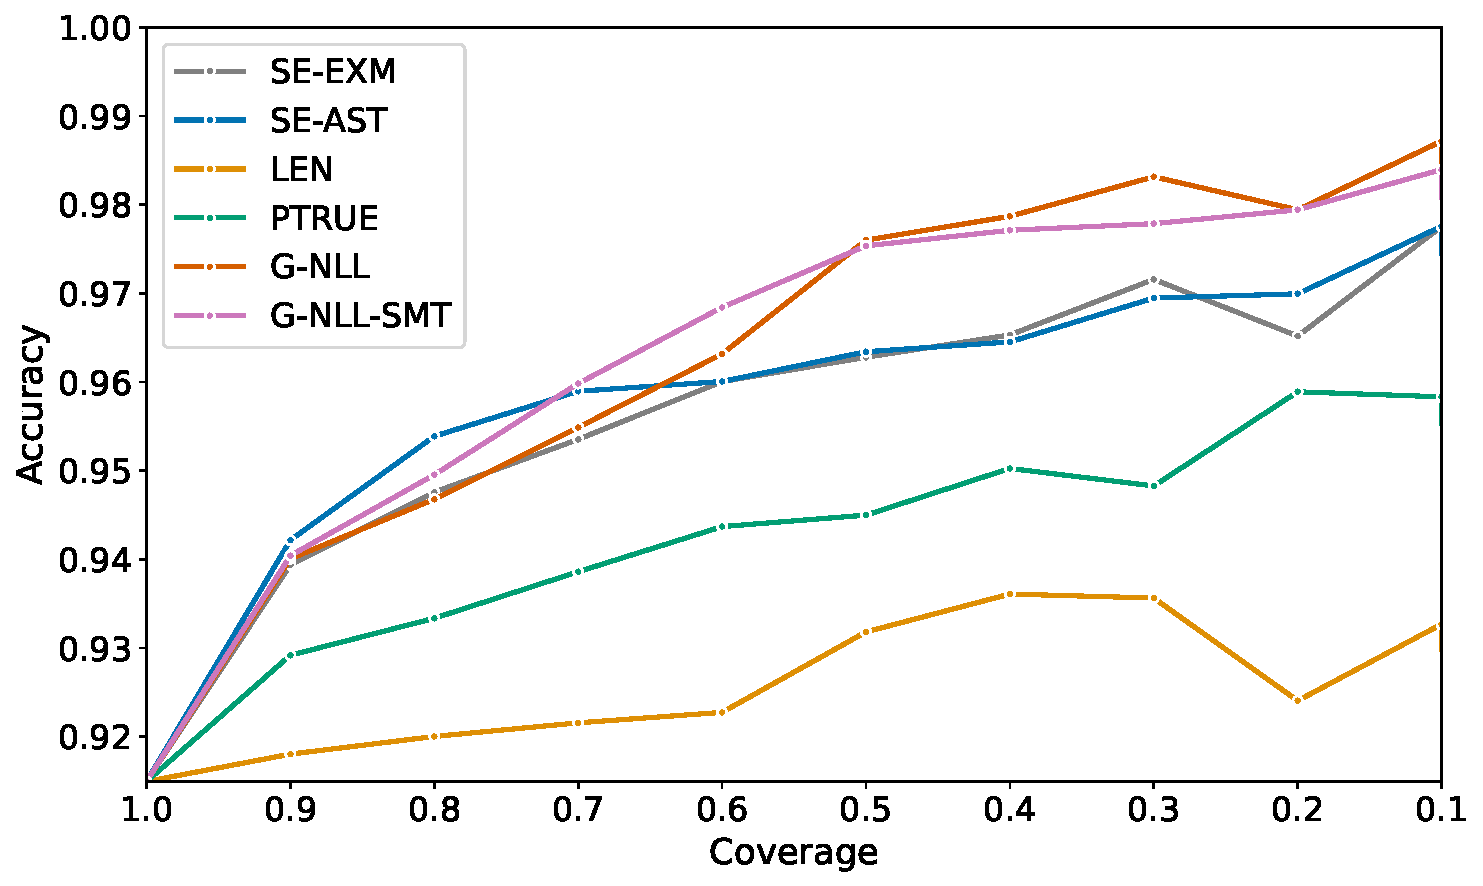
\includegraphics[width=\textwidth]{figures/rejection/simple_selective_accuracy_mean.pdf}
        \caption{Simple}
        \label{fig:Simple_rc}
    \end{subfigure}
    \hfill
    \begin{subfigure}[c]{0.48\textwidth}
        \centering
        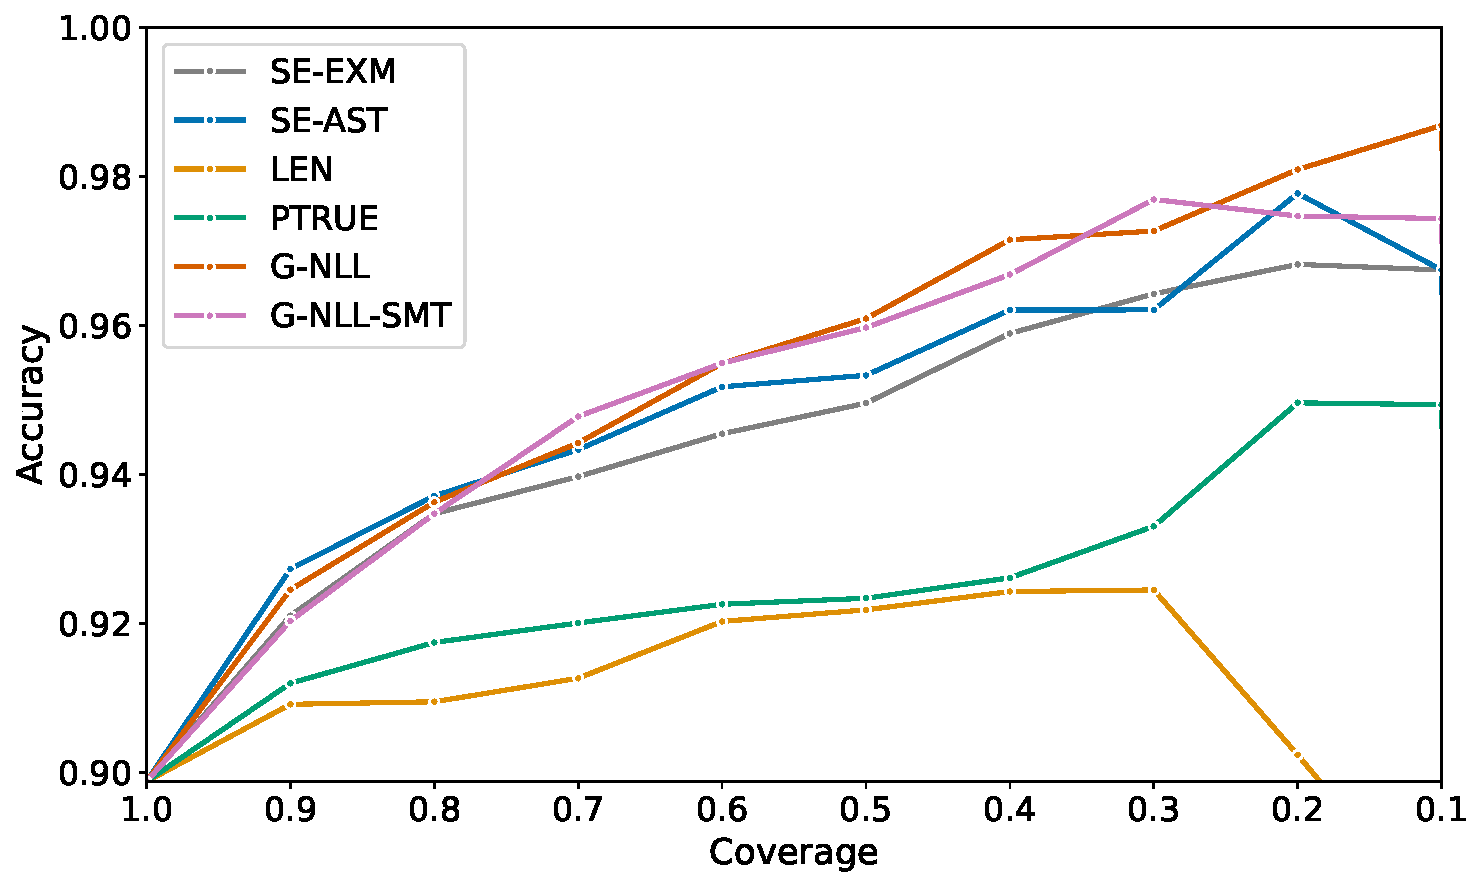
\includegraphics[width=\textwidth]{figures/rejection/multiple_selective_accuracy_mean.pdf}
        \caption{Multiple}
        \label{fig:Multiple_rc}
    \end{subfigure}
    
    \vskip\baselineskip

    \begin{subfigure}[c]{0.48\textwidth}
        \centering
        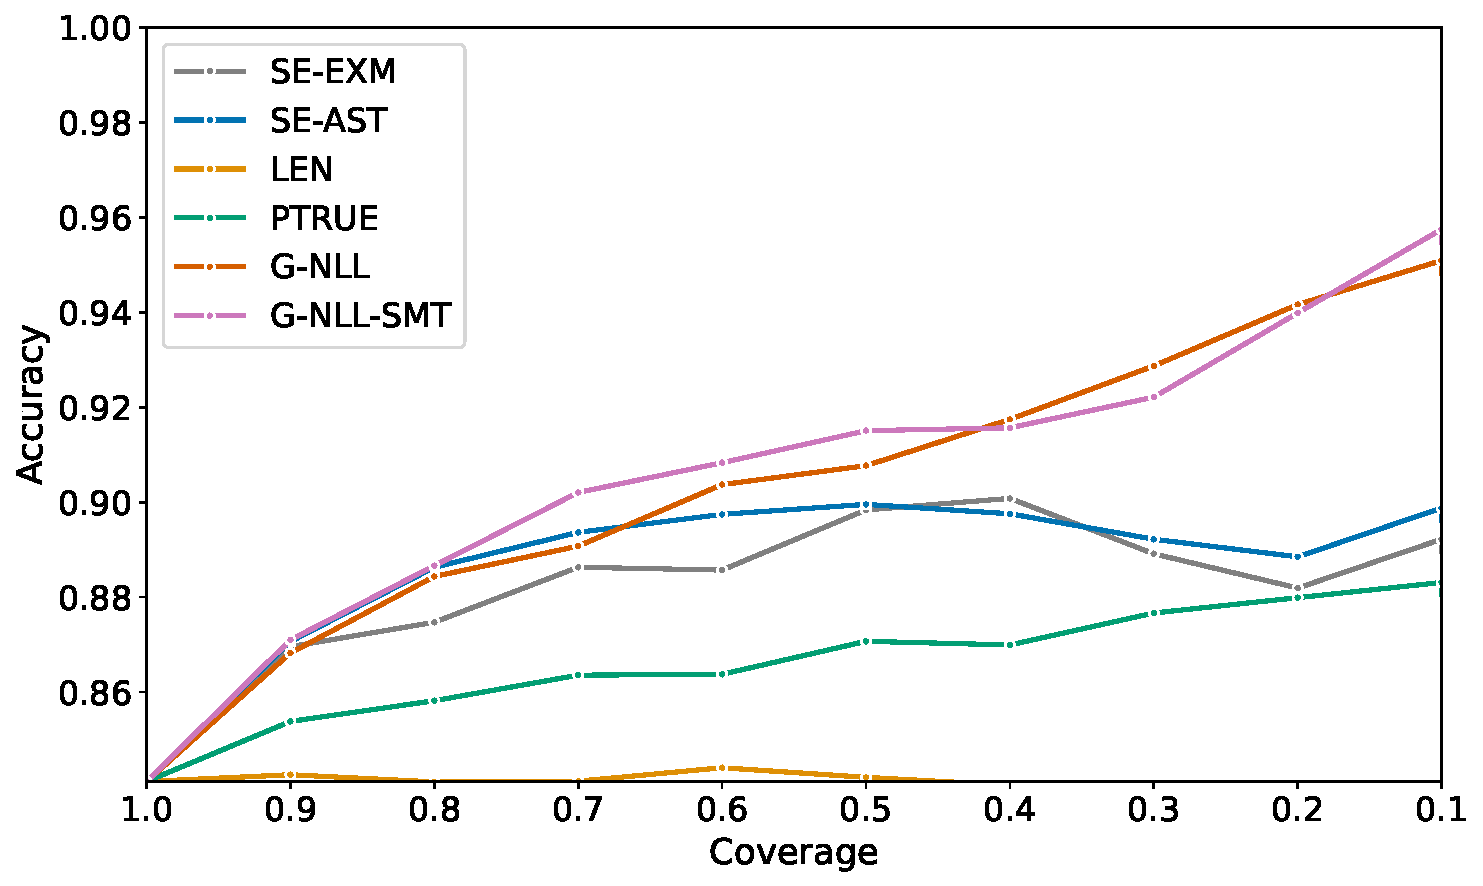
\includegraphics[width=\textwidth]{figures/rejection/parallel_selective_accuracy_mean.pdf}
        \caption{Parallel}
        \label{fig:Parallel_rc}
    \end{subfigure}
    \hfill
    \begin{subfigure}[c]{0.48\textwidth}
        \centering
        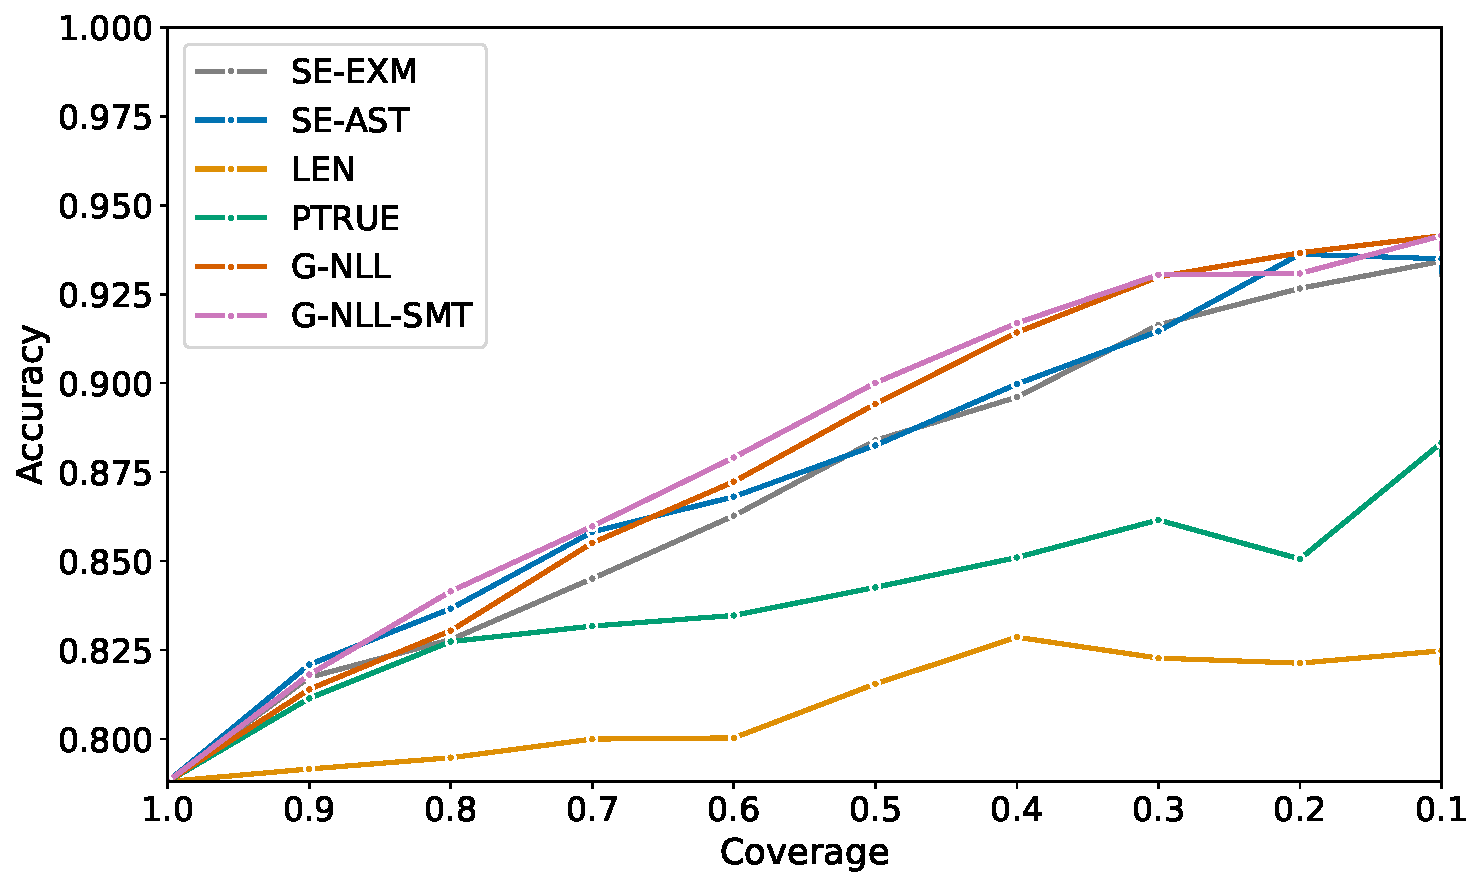
\includegraphics[width=\textwidth]{figures/rejection/parallel_multiple_selective_accuracy_mean.pdf}
        \caption{Parallel-Multiple}
        \label{fig:Parallel-Multiple_rc}
    \end{subfigure}

    \caption{
        Individual tasks: 
        Risk-coverage curves for the individual tasks described in \Cref{sec:individual_tasks}, averaged across models. Higher is better.
    }
    \label{fig:individual_tasks_riskcoverage}
\end{figure*}



\begin{figure*}[h!]
    \centering
        \begin{subfigure}[c]{0.48\textwidth}
        \centering
        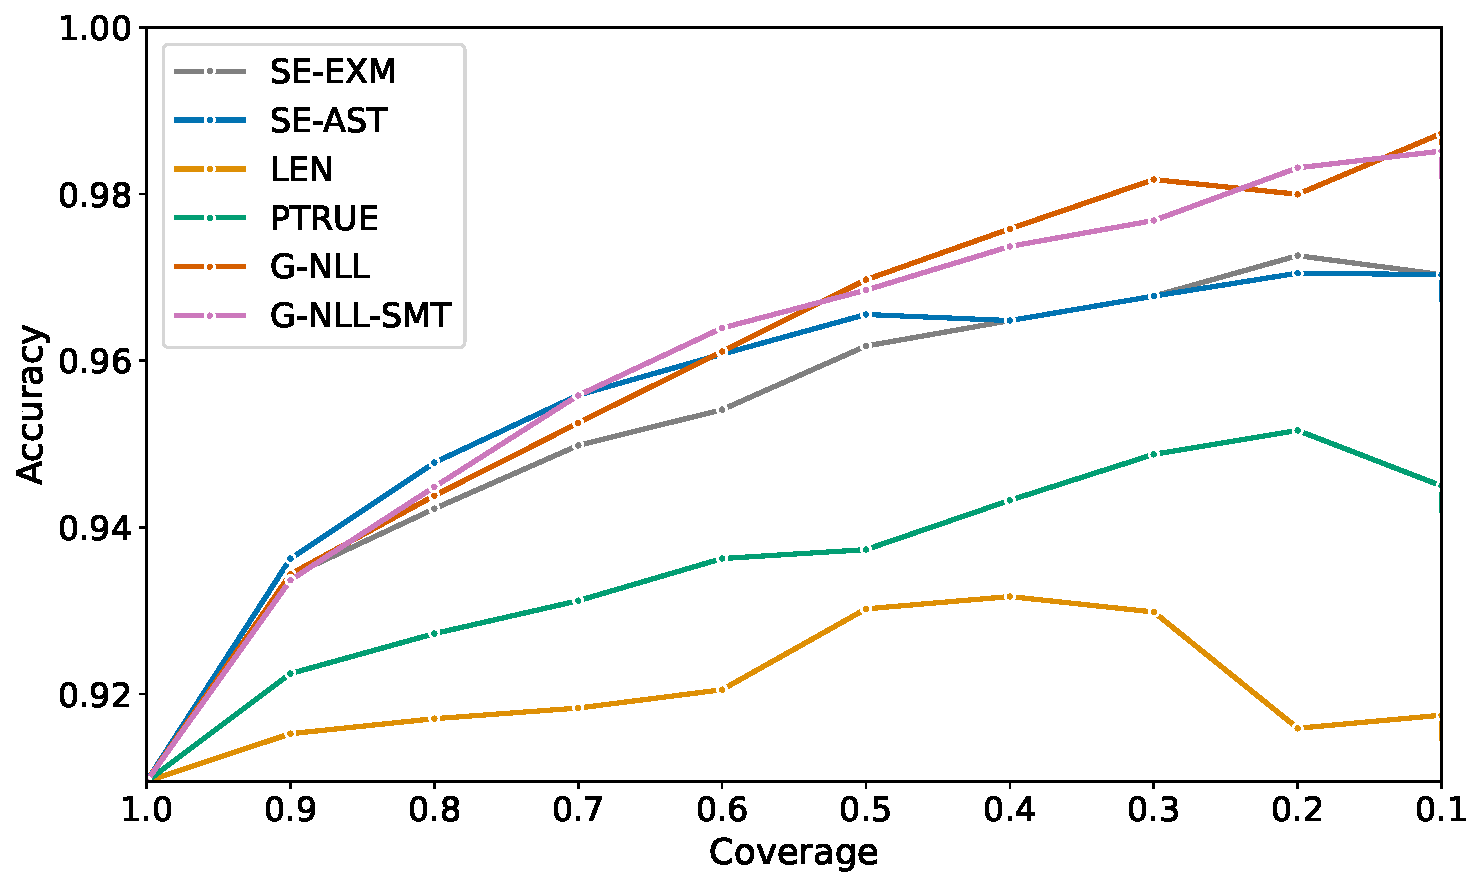
\includegraphics[width=\textwidth]{figures/rejection/simple-multiple_selective_accuracy_mean.pdf}
        \caption{Simple + Multiple}
        \label{fig:Simple+Multiple_rc}
    \end{subfigure}
    \hfill
    \begin{subfigure}[c]{0.48\textwidth}
        \centering
        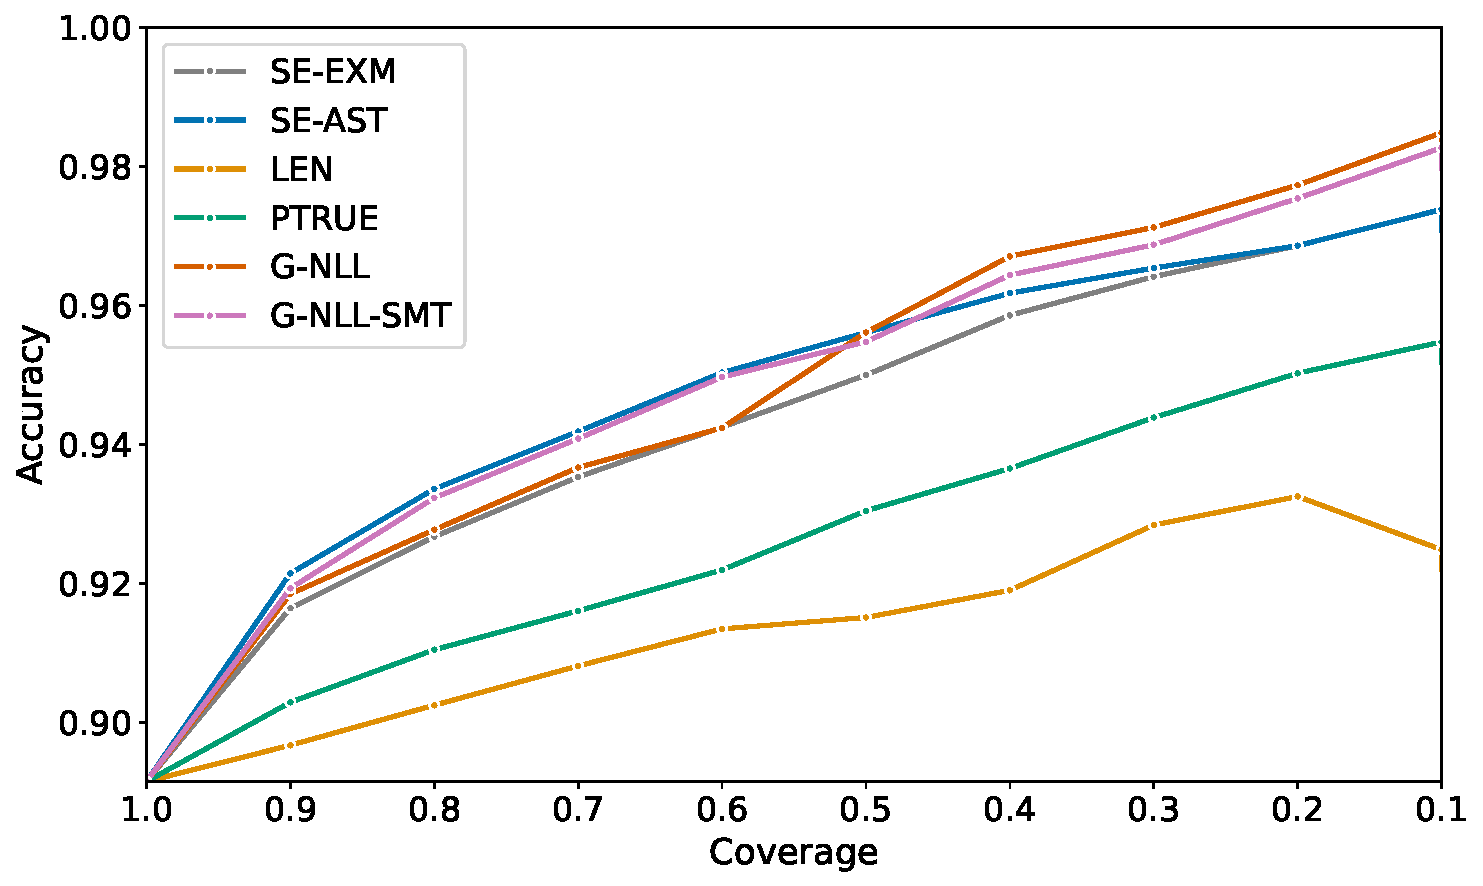
\includegraphics[width=\textwidth]{figures/rejection/simple-parallel_selective_accuracy_mean.pdf}
        \caption{Simple + Parallel}
        \label{fig:Simple+Parallel_rc}
    \end{subfigure}

    \vspace{0.5em}

    \begin{subfigure}[c]{0.48\textwidth}
        \centering
        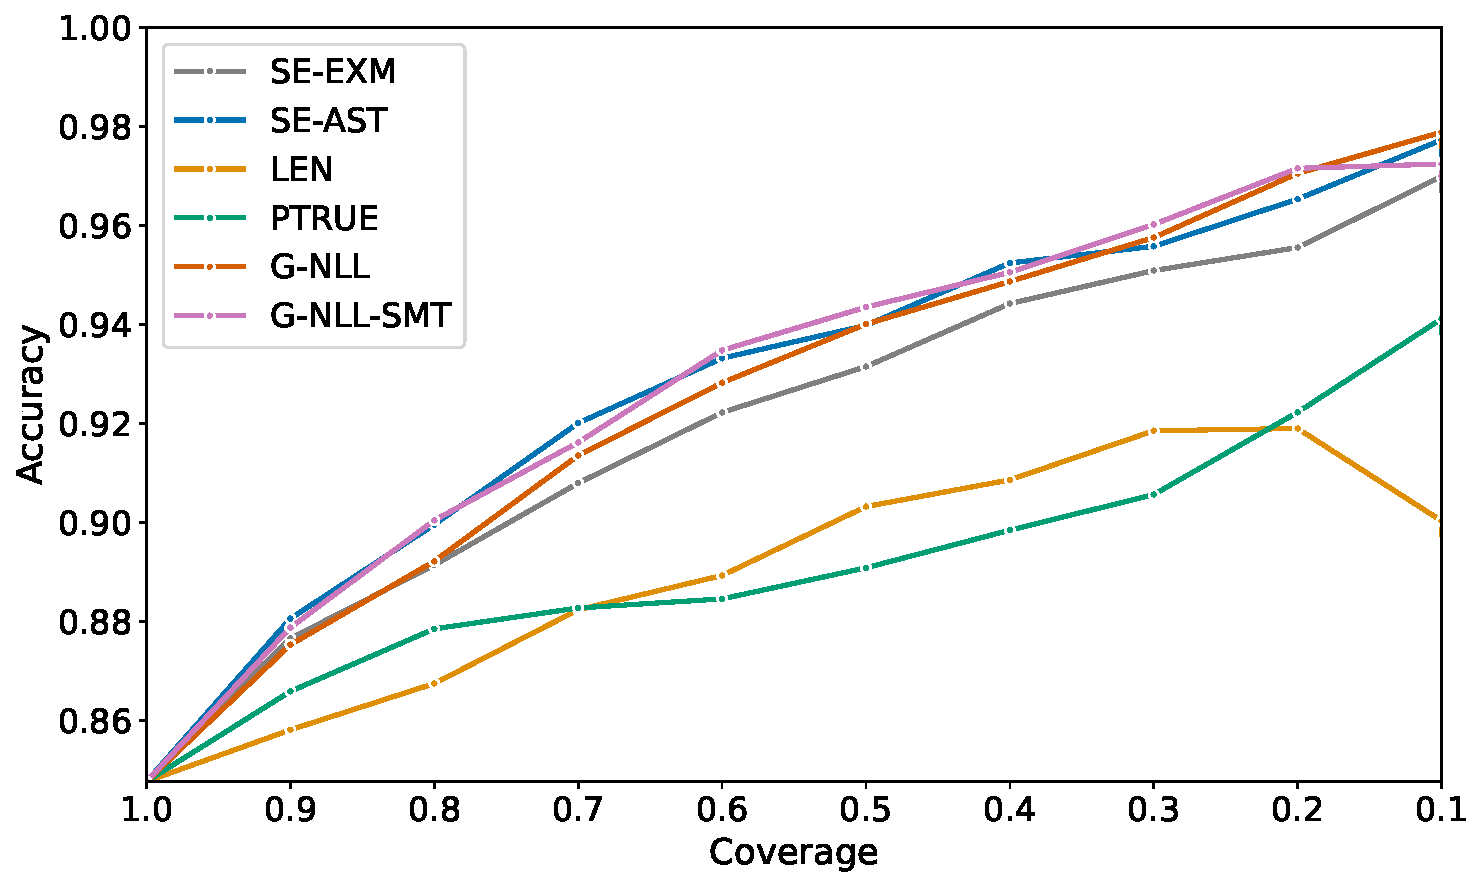
\includegraphics[width=\textwidth]{figures/rejection/multiple-parallel_multiple_selective_accuracy_mean.pdf}
        \caption{Multiple + \mbox{Parallel-Multiple}}
        \label{fig:Multiple+Parallel-Multiple_rc}
    \end{subfigure}
    \hfill
    \begin{subfigure}[c]{0.48\textwidth}
        \centering
        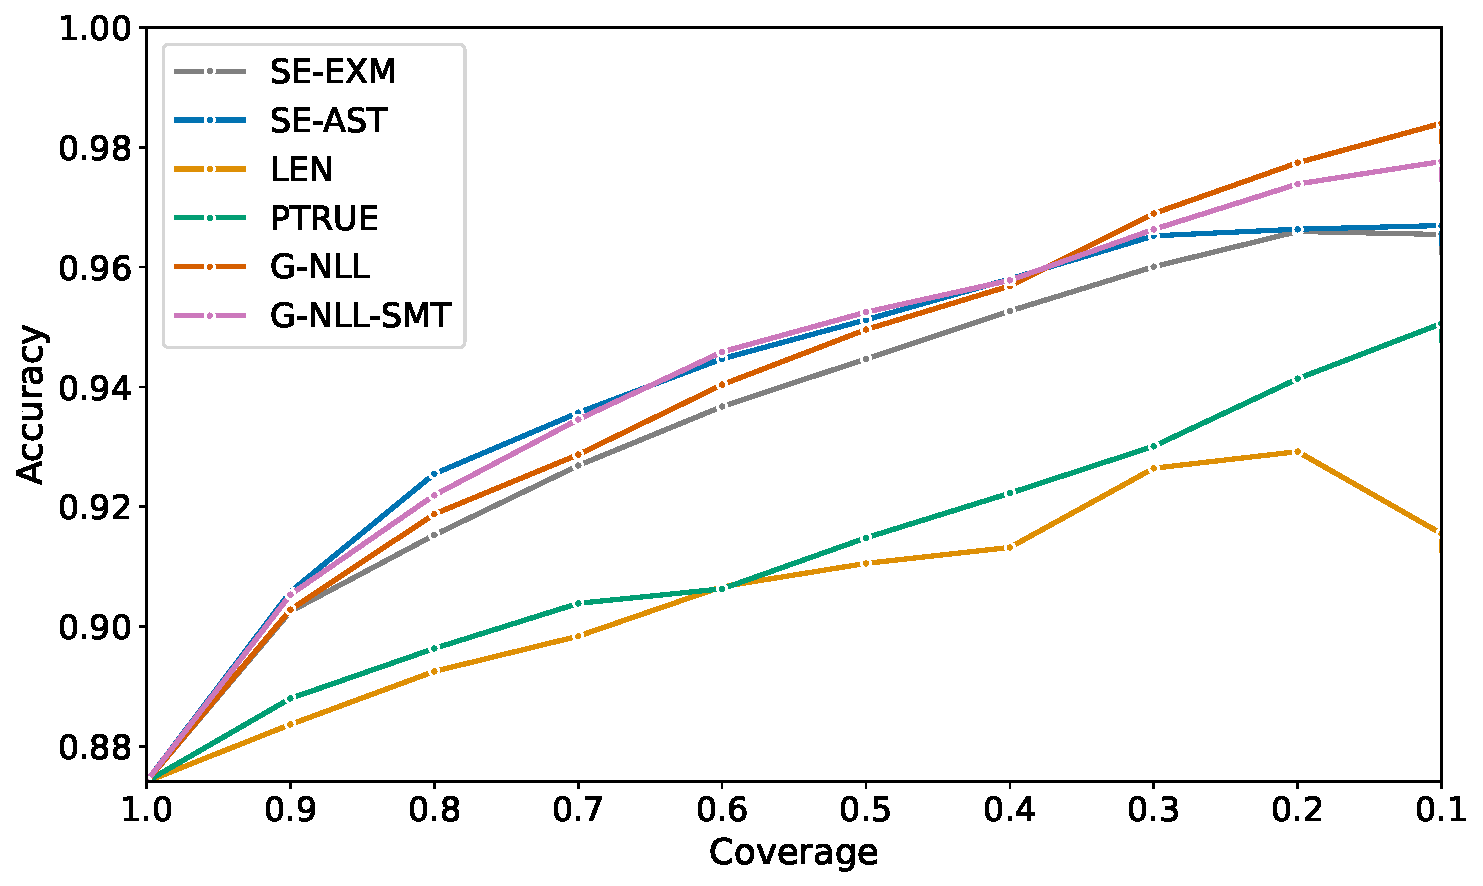
\includegraphics[width=\textwidth]{figures/rejection/simple-multiple-parallel-parallel_multiple_selective_accuracy_mean.pdf}
        \caption{All Combined}
        \label{fig:All_rc}
    \end{subfigure}

    \caption{
        Combination of tasks: 
        Risk-coverage curves for the combinations of tasks described in \Cref{sec:combinations}, averaged across models. Higher is better.
    }
    \label{fig:combined_tasks_riskcoverage}
\end{figure*}


\begin{figure*}[h!]
\centering
    \begin{subfigure}[c]{0.48\textwidth}
        \centering
        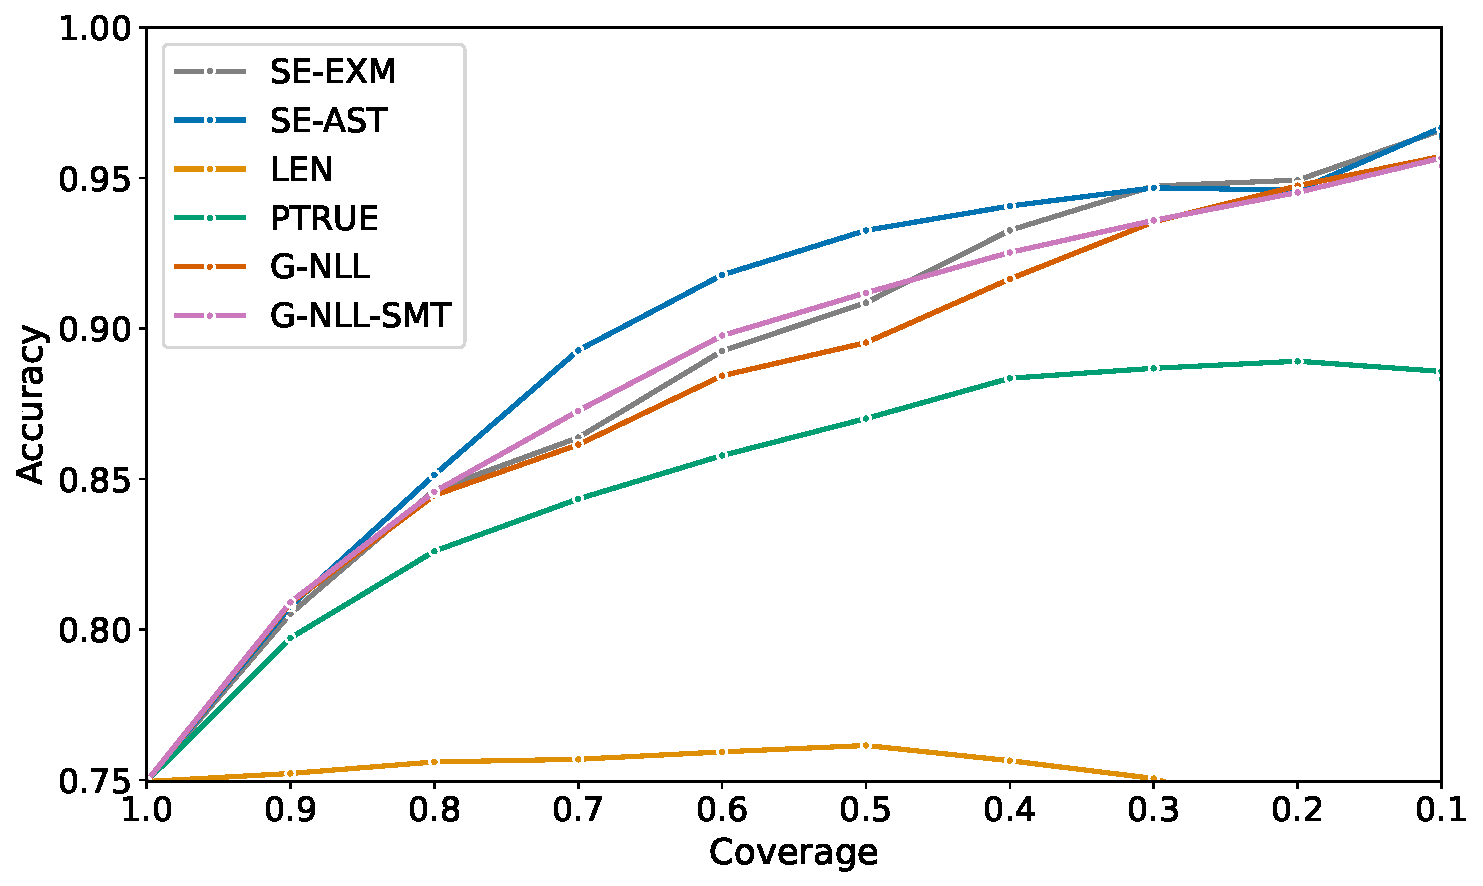
\includegraphics[width=\textwidth]{figures/rejection/simple-irrelevance_selective_accuracy_mean.pdf}
        \caption{Simple + Irrelevance}
        \label{fig:Simple+Irrelevance_rc}
    \end{subfigure}
    \hfill
    \begin{subfigure}[c]{0.48\textwidth}
        \centering
        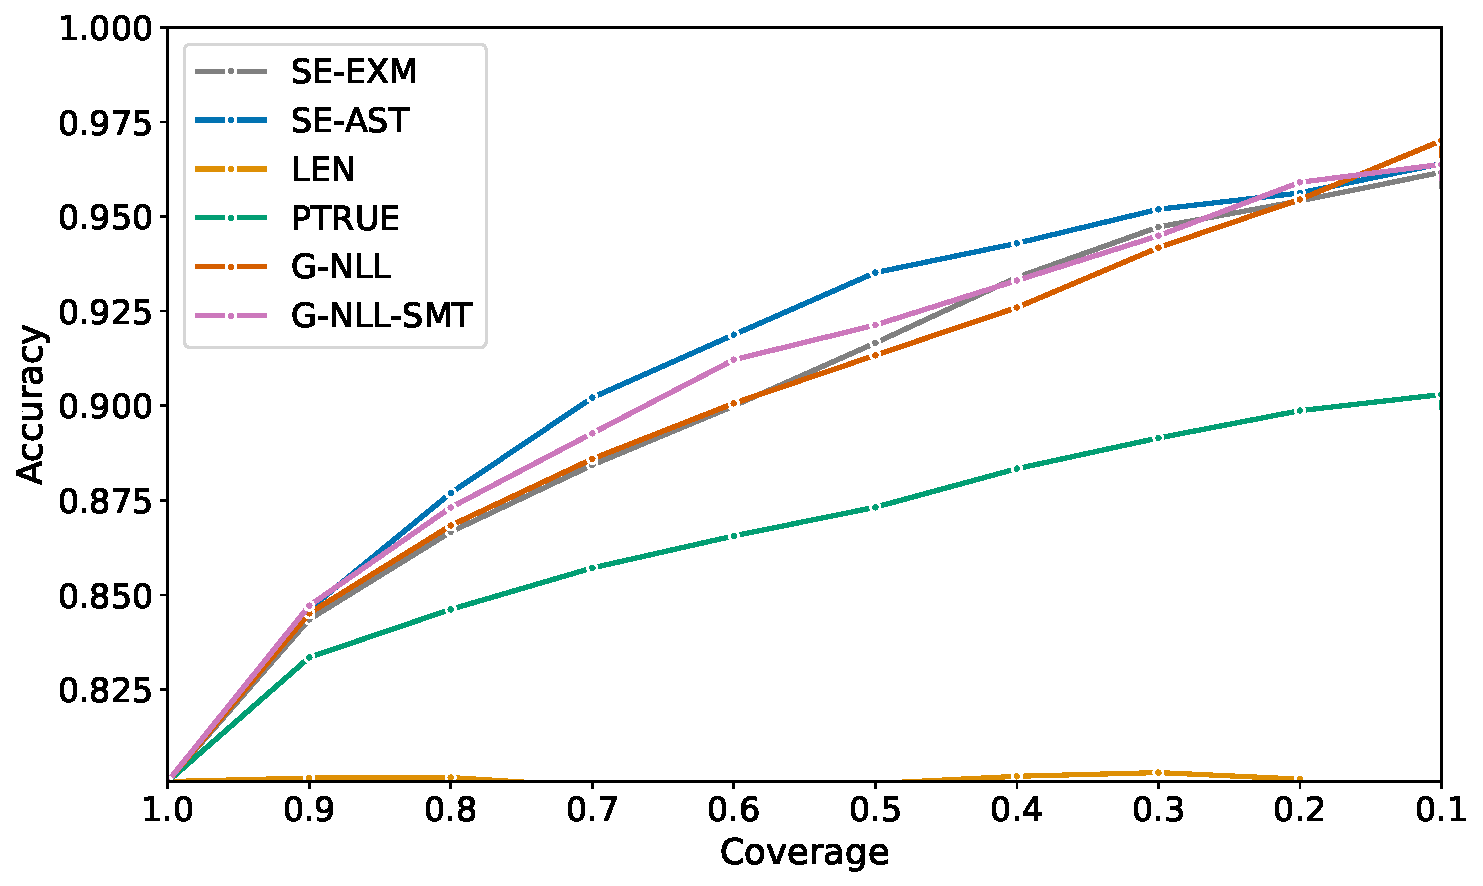
\includegraphics[width=\textwidth]{figures/rejection/simple-multiple-parallel-parallel_multiple-irrelevance_selective_accuracy_mean.pdf}
        \caption{All Combined + Irrelevance}
        \label{fig:All+Irrelevance_rc}
    \end{subfigure}

    \caption{
        Unanswerable requests: 
        Risk-coverage curves for the combinations of answerable and unanswerable tasks described in \Cref{sec:irrelevance_combinations}, averaged across models. Higher is better.
    }
    \label{fig:irrelevance_combinations_riskcoverage}
\end{figure*}




\subsection{Detailed Calibration Results}
\label{app:calibration}

In \Cref{fig:smoothECE_all} we show the calibration results for all individual and combined task datasets for \textbf{MAX}, \textbf{MAX}$_{SMT}$, \textbf{AVG}, \textbf{AVG}$_{SMT}$, \textbf{G-NLL}, \textbf{G-NLL}$_{SMT}$, and \textbf{P}$_{true}$. Other UQ methods do not output probabilities, and their calibration can as such not be evaluated. 

\begin{figure*}[h!]
    \centering
        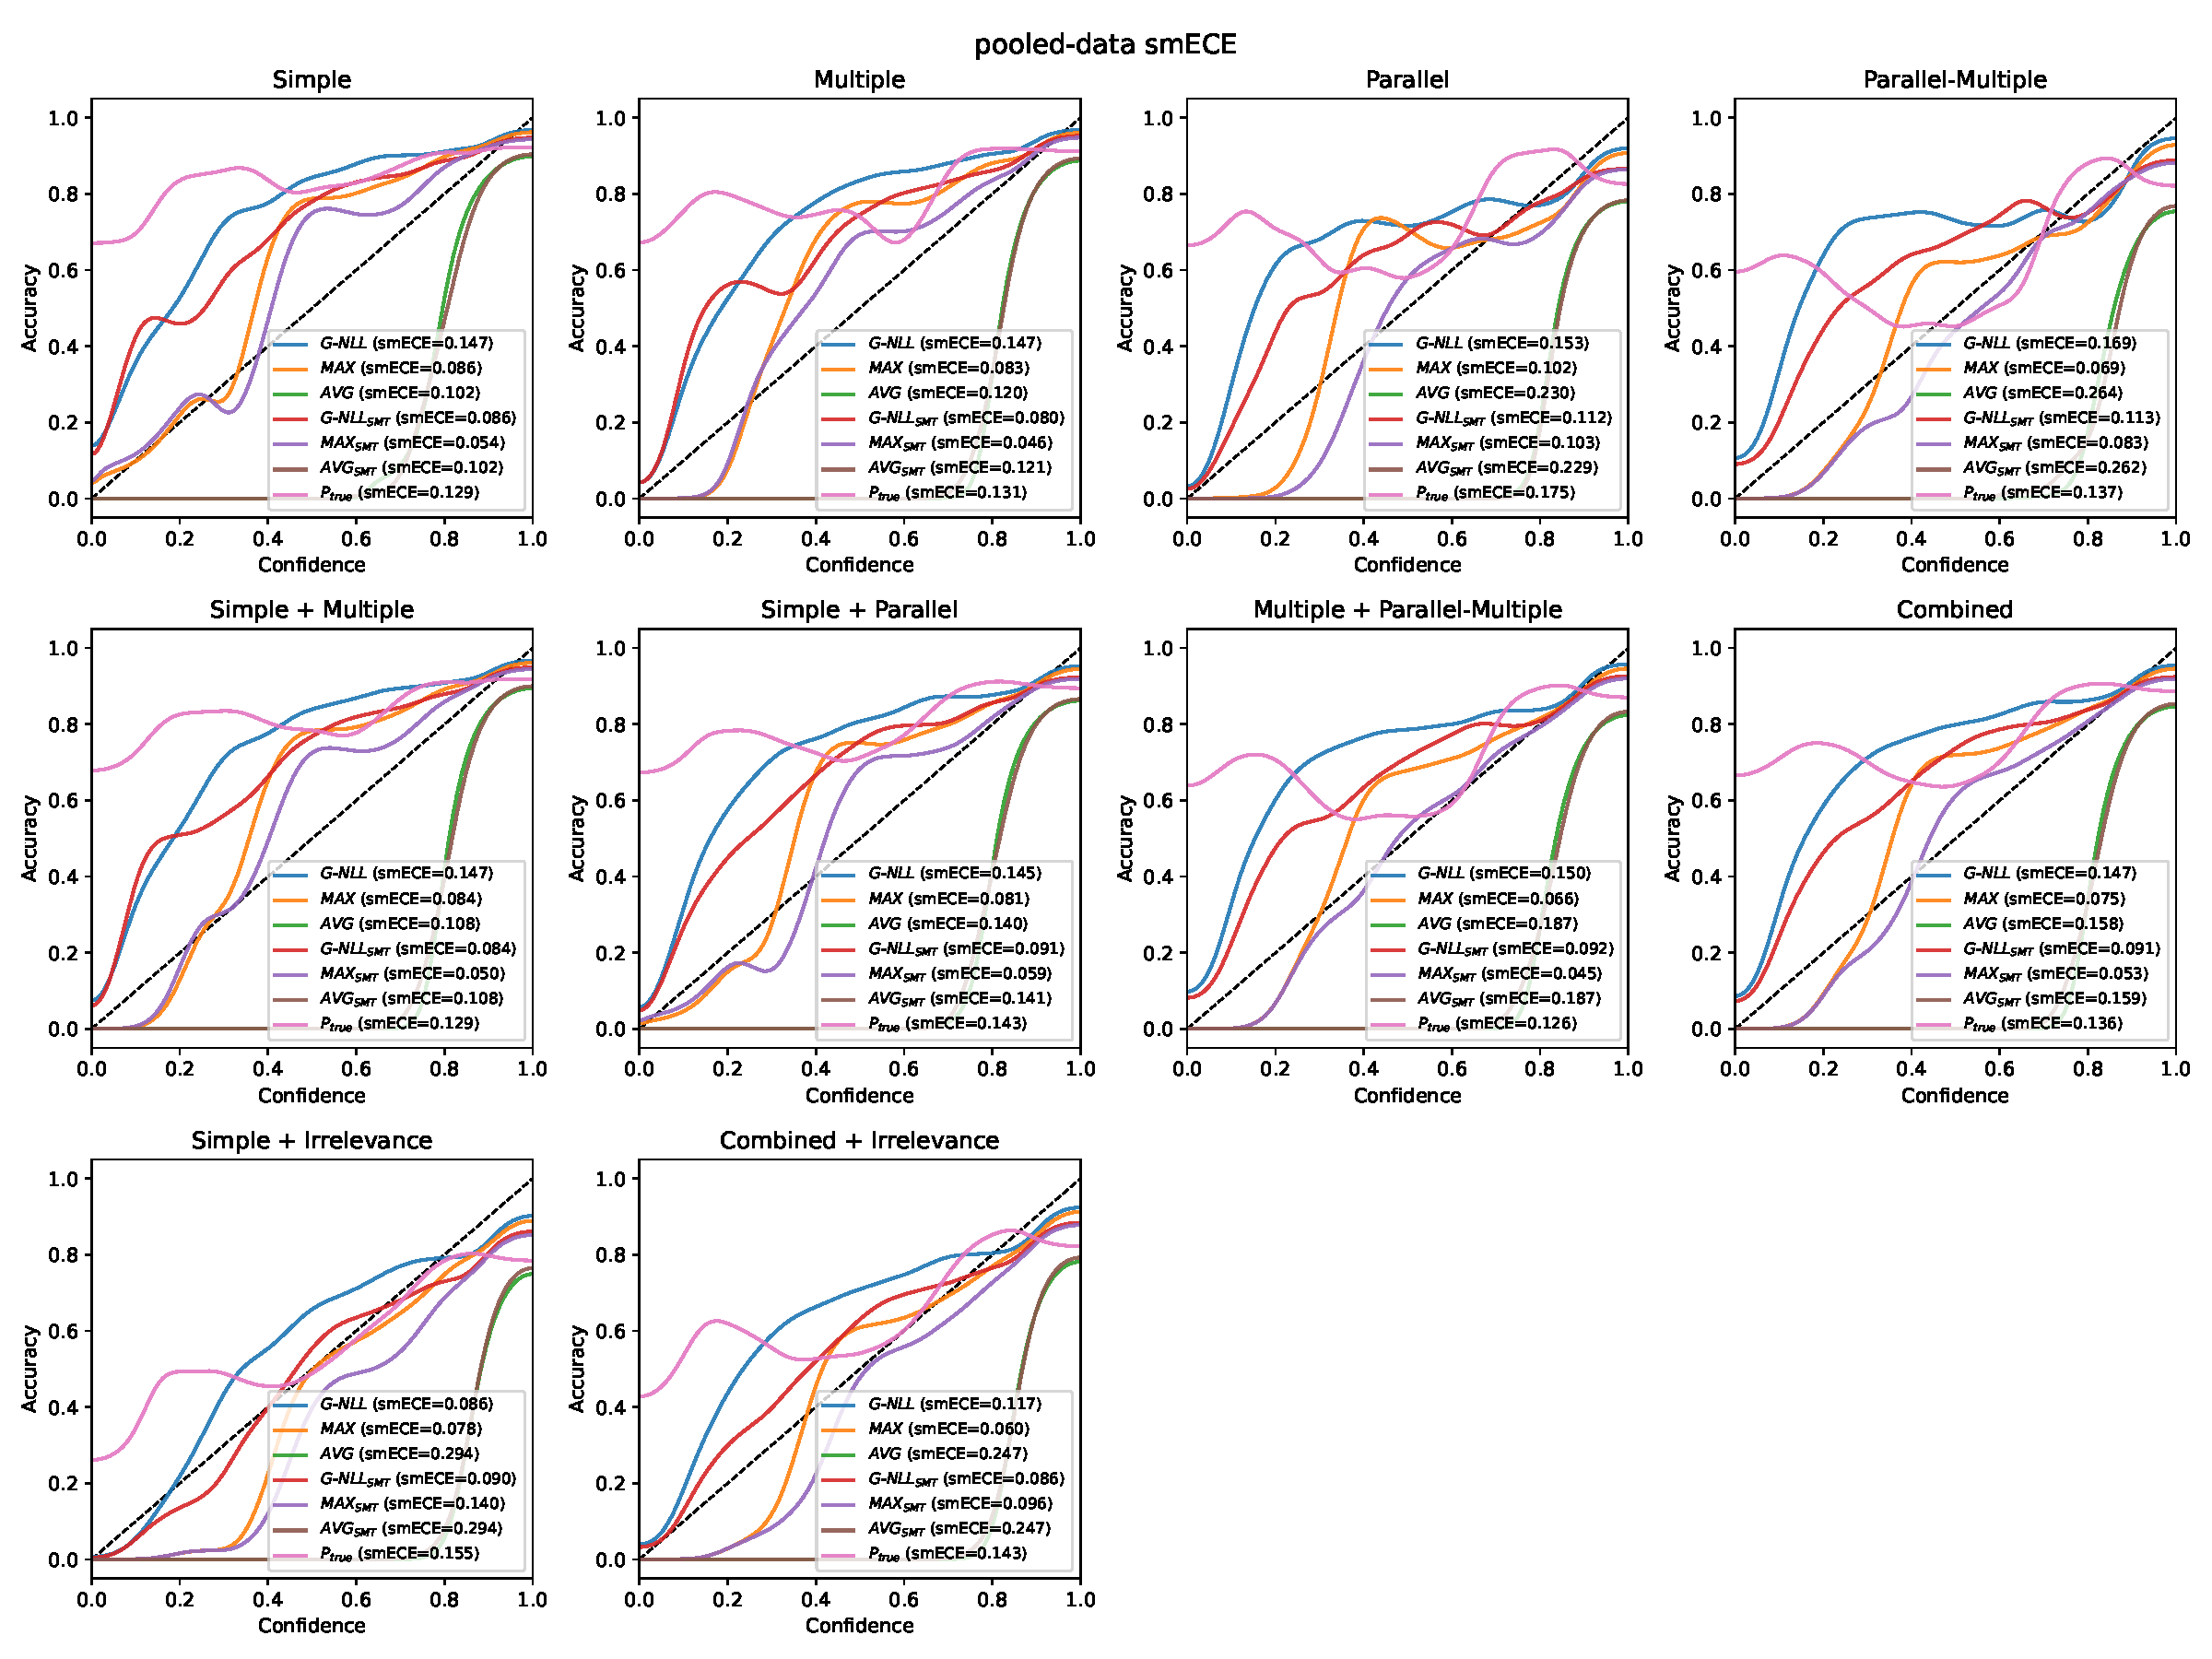
\includegraphics[width=\textwidth, trim=10 10 10 35, clip]{figures/ece/calibration_pooled_v2.pdf}
    \caption{
        SmoothECE for all tasks aggregated over models.
    }
    \label{fig:smoothECE_all}
\end{figure*}



\subsection{Post-hoc Calibration}
\label{app:posthoc}

As noted in \Cref{sec:calibration}, post-hoc calibration techniques can be applied to a UQ score after the fact. It is worth making precise what this can and cannot change about our conclusions. All of the discrimination and selective-prediction metrics we report---AUROC, as well as the NAURC and PRR results in \Cref{app:selection_pred_metrics}---depend on the UQ scores only through the ranking they induce. Any \emph{strictly} monotone map applied to the scalar uncertainty score, as Platt scaling and score-level temperature scaling are, therefore leaves all of these metrics exactly invariant. Rescaling the token logits before aggregation is not a map of this form, since it can reorder sequences of different lengths, and we leave logit-level recalibration to future work. Isotonic regression and histogram binning are only weakly monotone, and can affect rank-based metrics solely through the ties they introduce. Consequently, post-hoc calibration changes \emph{how} a given uncertainty score should be thresholded, which matters when choosing an abstention threshold for deployment, but it cannot change \emph{which} score is preferable, which is the question our benchmark is designed to answer. The converse also holds: because post-hoc calibration is by construction designed to reduce ECE, it would compress the smoothECE differences reported in \Cref{sec:calibration}, so it is the calibration comparison between methods---rather than the discrimination comparison---that a calibration step would change. We report uncalibrated values because they characterise the scores as they are produced by the model.

Which methods are amenable to monotone recalibration can be read off \Cref{fig:calibration}. The reliability curves of {G-NLL} and {MAX} are close to monotone, and {AVG} is monotone although nearly flat over most of its range, so all three should recalibrate well. {P}$_{true}$, by contrast, is clearly non-monotone: its accuracy rises to $\approx\!0.75$ around a confidence of $0.2$, falls to $\approx\!0.63$ around $0.5$, peaks near $0.90$ around $0.8$, and then declines. No monotone map can calibrate such a score, and doing so would require a binning-based map, which would in turn degrade its ranking performance. This is consistent with the comparatively weak AUROC of {P}$_{true}$ throughout \Cref{sec:benchmark}.
